% Grundgröße 12pt, zweiseitig
\documentclass[12pt,a4paper,twoside,parskip=half-,headsepline,headinclude]{scrreprt}
% Seitenköpfe automatisch
\usepackage[headsepline,automark]{scrpage2}
% Sprachpaket für Deutsch (Umlaute, Trennung, deutsche Überschriften)
\usepackage[ngerman]{babel}
\usepackage{blindtext}
% Graphikeinbindung, Hyperref (alles klickbar, Bookmarks),
\usepackage{graphicx, hyperref, amssymb}
% Umlaute - nochmal, die oben gehen nicht...
\usepackage[utf8]{inputenc}
% Math (Symbole aus AmsTeX)
\usepackage{amsmath}
% Einbindung von Code
\usepackage{listings}
% Farben
\usepackage{color}
% Fun with neural nets
\usepackage{tikz}
% Listen
\usepackage{enumerate}
% File explorer
\usepackage{dirtree}
% Korrekte Anführungszeichen
\usepackage{csquotes}

% Farben (für Codelistings)
\definecolor{mygreen}{rgb}{0,0.6,0}
\definecolor{mygray}{rgb}{0.3,0.3,0.3}
\definecolor{mymauve}{rgb}{0.58,0,0.82}

\newcommand{\todo}[1]{\textcolor{red}{TODO: {#1}}}

% Genereller Style für Codelistings
\lstset{ %
  backgroundcolor=\color{white},
  breakatwhitespace=false,
  basicstyle=\small\sffamily,
  breaklines=true,
  captionpos=b,
  commentstyle=\color{mygreen},
  escapeinside={\%*}{*)},
  extendedchars=true,
  keepspaces=true,
  keywordstyle=\color{blue},
  language=Octave,
  morekeywords={__shared__, __global__, until, each, synchronize threads},
  numbers=left,
  numbersep=5pt,
  numberstyle=\small\color{mygray},
  rulecolor=\color{black},
  showspaces=false,                
  showstringspaces=false,
  showtabs=false,
  stepnumber=1,
  stringstyle=\color{mymauve},
  tabsize=2
}

% Optionen für neuronale Netze
\def\layersep{3.0cm}
\def\layersepN{3.5cm}

% Festlegung Kopf- und Fußzeile     
\defpagestyle{meinstil}{%
	{\headmark \hfill}
	{\hfill \headmark}
	{\hfill \headmark\hfill }
	(\textwidth,.4pt)
}{%
	(\textwidth,.4pt)
	{\pagemark\hfill Alexander-Sebastian Clauß}
	{Version 0.9 vom \today\hfill \pagemark}
	{Version 0.9 vom \today\hfill\pagemark} 
}
\pagestyle{meinstil} 

\raggedbottom
\renewcommand{\topfraction}{1}
\renewcommand{\bottomfraction}{1}

 
%%%%%%%%%%%%%%%%%%%%%%%%%%%%%%%%%%%%%%%%%%%%%%%%%%%%%%%%%%%%%%%%%%%%%%%%%
%							hier gehts los								%
%%%%%%%%%%%%%%%%%%%%%%%%%%%%%%%%%%%%%%%%%%%%%%%%%%%%%%%%%%%%%%%%%%%%%%%%%

\begin{document}    
  \thispagestyle{empty} % Titelseite

\includegraphics[width=0.2\textwidth]{images/hsh_wortmarke.pdf}
{ \sffamily
  \vfill
  {
    \Huge\bfseries Unsupervised Image Clustering
  }
  \bigskip

  {
    \Large 
  	Alexander-Sebastian Clauß \\[2ex]
 	Master-Arbeit im Studiengang "`Angewandte Informatik"' 
    \\[5ex]
    \today 
  } 
}
\vfill
\hfill


\includegraphics[height=0.3\paperheight]{images/hsh_logo.pdf} 

\vspace*{-3cm}

\newpage \thispagestyle{empty}
\begin{tabular}{ll}
{\bfseries\sffamily Autor} & Alexander-Sebastian Clauß \\ 
            			   & Matrikelnummer: 1381164 \\
            			   & alexander-sebastian.clauss@hs-hannover.de \\[5ex]
{\bfseries\sffamily Erstprüferin:} & Prof. Dr. Frauke Sprengel \\
          						   & Abteilung Informatik, Fakultät IV \\
         						   & Hochschule Hannover \\
        						   & frauke.sprengel@hs-hannover.de \\[5ex]
{\bfseries\sffamily Zweitprüfer:}  & Maximilian Zubke \\
          						   & Abteilung Information und Kommunikation, Fakultät III \\
         						   & Hochschule Hannover \\
        						   & maximilian.zubke@hs-hannover.de
\end{tabular}

\vfill

% fett und zentriert in der minipage
\begin{center} \sffamily\bfseries Selbständigkeitserklärung \end{center}

Hiermit erkläre ich, dass ich die eingereichte Master-Arbeit
selbständig und ohne fremde Hilfe verfasst, andere als die von mir angegebenen Quellen und Hilfsmittel nicht benutzt und die den benutzten Werken wörtlich oder
inhaltlich entnommenen Stellen als solche kenntlich gemacht habe. 
\vspace*{7ex}

Hannover, den \today \hfill Unterschrift

\pdfbookmark[0]{Inhalt}{contents}

\tableofcontents
\listoffigures
\listoftables

\chapter{Einleitung}

TODO

\section{Motivation}

TODO

\section{Ziele der Arbeit}

TODO

\section{Aufbau und Ablauf}

TODO
\chapter{Grundlagen}

Das Grundlagenkapitel gibt eine Einführung und Übersicht über die verwendeten Begriffe und Konzepte, auf die im Weiteren der Arbeit zurückgegriffen wird. Zunächst wird die Darstellung von Bildern behandelt und anschließend die Erhebung von charakteristischen Merkmalen aus Bildern, den Features. Zur Detektion und Extraktion von Features aus Bildern haben sich zahlreiche verschiedene Verfahren etabliert. Von diesen wird der SIFT Feature Detektor und Deskriptor näher betrachtet, da er im Weiteren als Basis für die Feature Gewinnung dient. 
Es werden anschließend zwei Modelle vorgestellt, die eine Klassifikation von Bildern auf Basis von Features ermöglichen. Das Bag of Visual Words Modell wurde aus dem Bereich Information Retrival adaptiert. Es wird anhand der Features von Trainingsbildern eins visuelles Vokabular gelernt, dass zur Klassifizierung von Bildern dient. Alternativ zu diesem Ansatz wird der Autoencoder vorgestellt. Ein Autoencoder ist ein spezielles neuronales Netzwerk, dass selbständig eine komprimierte Darstellung der Eingabe, in diesem Fall der Features, lernt. 
Im letzten Teil wird auf die Berechnung allgemein mathematischer Probleme auf Grafikkarten, das GPGPU Programming eingegangen. Durch den Einsatz von Grafikkarten können Berechnungen gerade bei großen Datenmengen stark beschleunigt werden, da diese massiv parallel auf den Daten arbeiten. Mit Nvidias cuda wird eine Sprache eingeführt, mit der sich Modelle wie der Bag of Visual Words und Autoencoder auf Nvidia Grafikkarten ausführen lassen.

\section{Bilder und Features}

Zunächst wird definiert wie ein Bild mathematisch aufgefasst wird um eine effiziente Verarbeitung zu ermöglichen. Jedes Verfahren erwartet ein Bild als Eingabe. Verändern Algorithmen ein Bild, so geben sie die bearbeite Version wieder aus. Bei Analysen hingegen wird ein Bild nicht verändert, es wird auf Muster untersucht und die gefundenen Eigenschaften zurückgegeben. Diese Eigenschaften werden Features genannt. Der Prozess der Featuregewinnung ist in Detektion und Extraktion unterteilt und wird im Anschluss behandelt.

\subsection{Bilder}

Bei einem digitalen Bild handelt es sich um eine Matrix $I(x, y)$. Die Anzahl der Spalten $m$ und Zeilen $n$ entspricht dabei den Dimensionen des Bildes in Pixeln. Hier bezeichnen $(x, y)$ diskrete Koordinaten der Matrix und somit die einzelnen Pixel des Bildes. Die Darstellung in Matrixform eignet sich  sehr gut für Transformationen und Analysen des Bildes. Solche Verfahren betrachten oft jeden Pixel und seine Nachbarschaft. Die direkte Nachbarschaft eines Pixels ist eine $3 \times 3$ Matrix (mit dem Pixel als Zentrum), die alle unmittelbar anliegenden Pixel beinhaltet.

$$
I(x, y) = \begin{bmatrix}
i_{0, 0}   & i_{0, 1}	& \dots	 & i_{0, n-1}   \\
i_{1, 0}   & i_{1, 1}   & \dots  & i_{1, n-1}   \\
\vdots	   & \vdots 	& \ddots & \vdots       \\
i_{m-1, 0} & i_{m-1, 1} & \dots	 & i_{m-1, n-1}
\end{bmatrix}
$$ 

Abhängig vom Typ des Bildes, besitzen die Pixel eine andere Struktur. In der Bilderverarbeitung und im Weiteren dieser Arbeit werden meist folgenden Arten von Bildern verwendet:
\begin{itemize}
	\item \textbf{Monochromatische Bilder} Diese Bilder werden nur in Graustufe dargestellt, daher besitzt ein Pixel genau einen Intensitätswert.
	\item \textbf{Multispektrale Bilder} Jeder Pixel besitzt einen Vektor an Werten. Im Falle eines Farbbildes enthält der Vektor drei Intensitätswerte für rot, grün und blau.
\end{itemize}
Die Intensität eines Pixels bzw. die Intensität seiner Vektoren wird mit acht Bit dargestellt und umfasst daher 256 mögliche Werte. Diese Werte werden im Folgenden normalisiert im Intervall $[0, 1]$ angegeben.

\begin{itemize}
	\item TODO: Grafik mit beliebigem Bild und Abbildung von Pixel in Raster mit Koordinaten (x, y) ? 
\end{itemize}

\subsection{Feature Detektion und Extraktion}

Um Bilder zu vergleichen werden charakteristische Merkmale dieser betrachtet, die sogenannten Features. Ein Feature ist ein allgemeiner Begriff und enthält je nach Verfahren unterschiedliche Informationen. Dies ist notwendig, da nicht nur die Position oder Intensität eines Pixels, sondern auch generelle Eigenschaften von Interesse sind. Globale Verfahren berücksichtigen bei der Bewertung jeden Pixel des Bildes gleichermaßen, lokale hingegen betrachten nur ein kleine Fenster des Bildes, also einen Pixel und seine Nachbarschaft. Die Suche nach globalen Merkmalen, die ein Bild charakterisieren, kann aber keine Objekte und Details im Bild berücksichtigen. Hierfür eignet sich die Extraktion von lokalen Features. Um Objekte aus unterschiedlichen Perspektiven und in verschiedenen Größen wieder zu erkennen, ist es notwendig, dass die Features affin invariant sind. Folgende Abbildung zeigt dasselbe Objekt, jedoch rotiert, skaliert und verschoben. Ein Algorithmus sollte mit hoher Wahrscheinlichkeit erkennen, dass es sich hier um dasselbe Objekt handelt.

BEISPIEL BILD

Die Gewinnung der Features ist in zwei Schritte aufgeteilt: 
\begin{itemize}
	\item \textbf{Detektion} Zuerst ermittelt ein Detektor Muster im Bild. Die untersuchten Muster sind abhängig vom Detektor Pixel, Linien oder Regionen einer Nachbarschaft. Hierfür wird jeder Pixel und seine Nachbarschaft betrachtet und entschieden ob es sich um einen \textit{key point} handelt. Ein Detektor gibt als Ergebnis alle Pixel zurück, bei denen es sich um {key points} handelt. Manche Verfahren geben zusätzlich zu den \textit{key points} auch Eigenschaften wie die Orientierung oder den Maßstab aus. Um praktisch einsetzbar zu sein, muss ein Detektor ein Feature, dass in verschiedenen Bildern auftaucht, zuverlässig erkennen. Hier sollte aber die angestrebte Allgemeinheit berücksichtigt werden: Ein Feature Detektor für medizinische Bilder kann spezieller Annahmen treffen, als einer für eine allgemeine Bildsuche.
	\item \textbf{Extraktion} Die Feature Extraktion erzeugt aus den vom Detektor gefundenen \textit{key points} den Deskriptor. Ein Feature Deskriptor ist eine kompakte Darstellung eines Features. Die \textit{key points} und deren Eigenschaften werden in Zahlen kodiert. Oft wird hier nicht nur ein Feature erzeugt, sondern ein Feature-Vektor, der auch Deskriptoren der Nachbarschaft des \textit{key points} enthält. Von einem Deskriptor ist es wünschenswert, dass er affin invariant ist. Somit kann das Feature auch erkannt werden, wenn das Bild rotiert, verschoben oder skaliert wurde.
\end{itemize}

Im Folgenden werden zwei Verfahren zur Feature Detektion und Extraktion vorgestellt, die sich in der Praxis bewährt haben und teilweise affine Invarianz aufweisen. Das Histogram of Oriented Gradients ist weit verbreiteter ein Feature Deskriptor, der sich im Breich der Objektdetektierung bewährt hat. SIFT ist ein von Lowe entwickeltes Verfahren zur Feature Extraktion und Detektion. Bei der Detektion von Features werden Rotationen, Skalierungen und Translationen von gefundenen Features erkannt und diese durch Den Deskriptor als ein Histogramm der Orientierungen dargestellt.\cite{ifd2016}

\begin{figure}
	\centering
	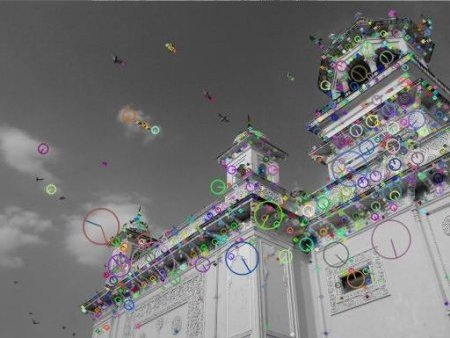
\includegraphics[scale=0.7]{images/sift_keypoints.jpg}
	\caption{Gefundene \textit{key points} in einem Bild farblich hervorgehoben (SIFT Detektor)}
	\label{img:interset_points}
\end{figure}

\subsection{Histogram of Oriented Gradients}

Um den Begriff zu klären, werden zunächst das Histogramm und Gradienten von Bildern (\textit{image gradients}) eingeführt. Ein Histogramm ist eine diskrete Funktion, welche die Häufigkeitsverteilung einer Menge abbildet. Hierfür wird jeder Wert der Menge einer Klasse zugeordnet. Jede Klasse umfasst einen vorher definierten Wertbereich. Als einfachen Fall dient hier die Verteilung der Pixel eines Bildes auf die Intensitäten. Bei einem monochromatischen Bild liegen 256 Klassen vor. Beim bilden des Histogramms wird jeder Punkt betrachtet und der Zähler der Klasse um eins inkrementiert, in deren Wertebereich der Intensitätswert des Punktes fällt. Ein Histogramm ist normalisiert, wenn die Anzahl der Werte einer Klasse durch die Anzahl der Gesamtwerte dividiert wird.
In Abbildung \ref{img:hist} sind im Wesentlichen zwei Bereiche zu erkennen: ein sehr hellerer Hintergrund und eine dunkle Katze, die den Großteil des Bildes ausmacht. Dies spiegelt sich auch im Histogramm wieder: Es ist eine große Mengen an Punkten im dunklen Bereich vorhanden (Intensität < 128) und eine kleine, extreme Häufung im hellen Bereich.

\begin{figure}
	\centering
	\includegraphics[scale=0.8]{images/big_cat.png}
	\caption{Graustufenbild und Verteilung der Intensitätswerte}
	\label{img:hist}
\end{figure}

Ein Gradient gibt die Intensitätsänderung eines Pixels und seiner Nachbarschaft in einer Richtung an. Die dominante Richtung entspricht einer großen Intensität. 

\begin{itemize}
	\item TODO: Histogram of Oriented Gradients
 	\item TODO: Abbildung
\end{itemize}

\subsection{Scale-invariant feature transform}

SIFT ist ein Feature Detektor und Deskriptor der 1999 von Lowe entwickelt wurde. Die von SIFT entdeckten Features sind (affin?) invariant und beschreiben die Nachbarschaft eines \textit{keypoints}. Der Algorithmus ist in vier Schritte unterteilt:

\begin{enumerate}
	\item \textbf{Detektion von Extremen im Maßstab} Die \textit{keypoints} werden durch einen Difference of Gaussians (DOG) Filter ermittelt. Das Bild wird durch eine Konvolution mit einem gausschen Kernel $G(x, y, d)$ geglättet, wobei $d$ die Standardabweichung ist. Dadurch das nur räumliche Informationen höherer Bereiche unterdrückt werden, fungiert dies als Band Pass Filter und hebt so die Sichtbarkeit von Kanten hervor. Der Lapalacien of Gaussian wird dann durch die Differenz zweier Gaussians berechnet. Dabei ist die Standardabweichung des Minuenden $k$ mal größer, als die des Subtrahenden. In der Praxis hat sich beim Einsatz in SIFT der Wert $k = 1.4$ bewährt. Die Extrempunkte aus einer Reihe von DOG Abbildungen sind dann die Punkte, die ein lokales Minimum oder Maximum besitzen. 
\begin{figure}
	\centering
	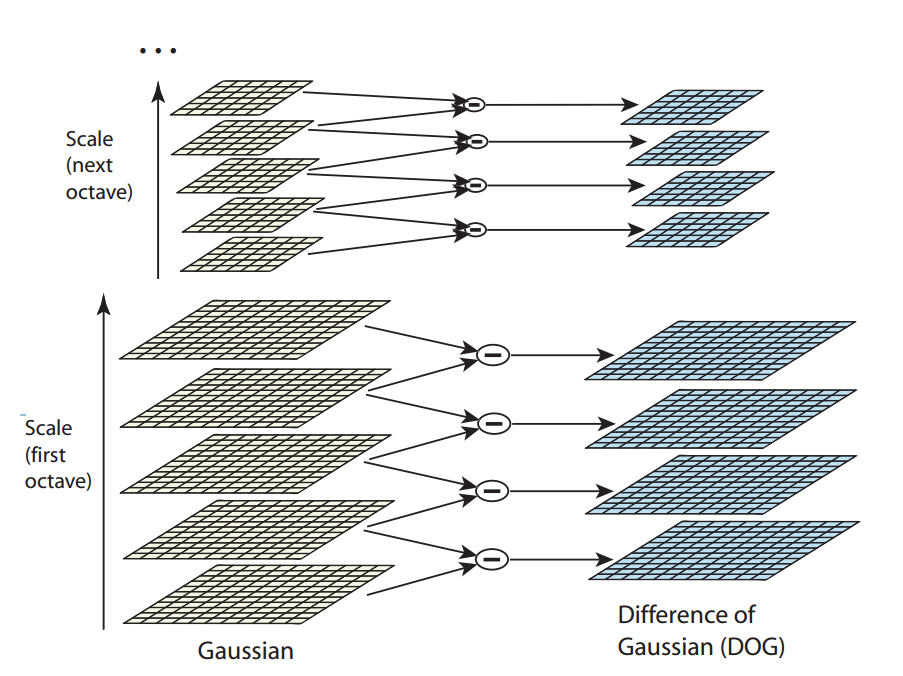
\includegraphics[scale=0.5]{images/sift_dog.png}
	\caption{Difference of Gaussians Operator, Abbildung aus \cite{dif2004}}
	\label{img:sift_dog}
\end{figure}	
	
	\item \textbf{Keypoint Lokalisierung} Nicht alle Kandidaten werden zu \textit{keypoints}. Jeder Kandidaten muss einer Reihe von Stabilitätsmaßen genügen. Befindet sich ein Punkt auf einer Kante oder besitzt einen zu geringen Kontrast, wird er aussortiert. Dies wird durch eine Taylor Expansion zweiter Ordnung mit Ursprung im \textit{keypoint} durchgeführt.
	\item \textbf{Bestimmung der Orientierung} Bei dem Aufbau des Feature Vektoren pro \textit{key points} wird die lokale Orientierung abgeschätzt. Auf diese Weise sind die SIFT Deskriptoren invariant gegenüber Rotationen. Der SIFT Algorithmus berechnet ein Histogramm der Orientierung der Gradienten. Hierfür werden zufällig Punkte aus der Nachbarschaft ausgewählt. Der Extremwert des Histogramms wird hier als dominante Orientierung verwendet.
	\item \textbf{Deskriptor} Für jeden durch den Detektor gefundenen \textit{keypoint} wird nun ein Featurevektor gebildet. Der Featurevektor enthält Informationen über die Nachbarschaft in Form der Gradienten eines jeden Punktes in der Nachbarschaft. Das Fenster für die Auswahl der Nachbarschaft wird auf dem \textit{keypoint} zentriert und in vier Teilfenster unterteilt. Die Gradienten in allen Teilfenster werden in acht Richtungen quantisiert, sodass der resultierende Deskriptor 128 Dimensionen enthält.
\begin{figure}
	\centering
	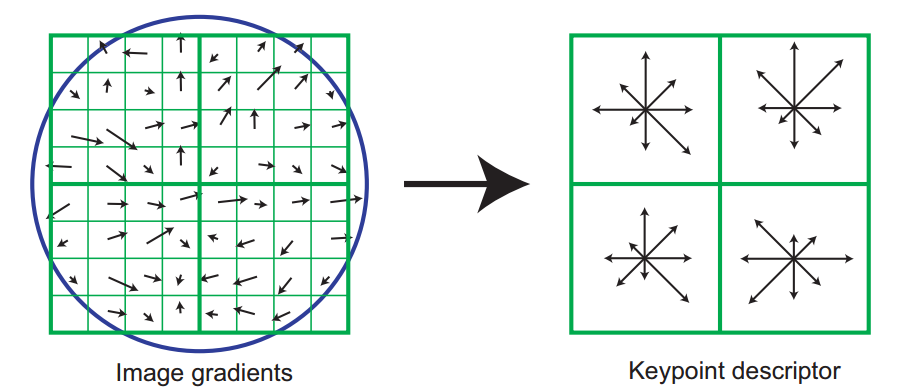
\includegraphics[scale=0.4]{images/sift_desc.png}
	\caption{Ein $8 \times 8$ Sample aus dem ein $2 \times 2$ Deskriptor berechnet wird, Abbildung aus \cite{dif2004}}
	\label{img:sift_desc}
\end{figure}	
	
\end{enumerate}

SIFT ist äußerst robust, da Änderungen im Grenzwert von Position und Orientierung den Feature Vektor kaum beeinflussen. Der Deskriptor besitzt zwar keine affine Invarianz, in praktischen Anwendungen werden jedoch auch mit skalierten, rotierten und verschobenen Objekten gute Ergebnisse erzielt. Auch im Vergleich zu anderen Algorithmen (SUSAN, SURF, ...) schneidet SIFT gut ab, meist mit besseren Ergebnissen. Die Konstruktion des Deskriptors ist allerdings sehr aufwendig und er weist eine hohe Dimensionalität auf. 

\begin{itemize}
	\item TODO: SIFT-PCA / Clustering erwähnen
	\item TODO: DOG näher erläutern, mathematische Notation?
\end{itemize}

\section{Bag of Visual Words}

Das Bag of Words Modell stammt aus dem Bereich Information Retrival und wird zur Klassifizierung von Dokumenten genutzt. Es wird das Auftreten jedes Wortes in eine Dokument gezählt und durch die Anzahl aller Wörter im Vokabular dividiert, um so einen normalisierten Wert zu erhalten, welcher die relative Häufigkeit eines Wortes angibt. Das Vokabular wird \textit{Codebook} genannt, die Wörter sind die \textit{Codewords}.
Dieses Modell wurde von der Computer Vision adaptiert um Bilder zu klassifizieren. Die Features können aber nicht direkt statt der Worthäufigkeit verwendent werden: Ein Wort ist ein diskreter Wert der direkt verglichen werden kann, ein Feature hingegen ist ein hochdimensionaler Vektor, der Eigenschaften beschreibt. Um konkrete Werte zu erhalten, ist es notwendig die Vektoren zu quantisieren. Die quantisierten Vektoren entsprechen dann den \textit{Codewords} und werden in diesem Kontext auch \textit{Visual Words} genannt. Um \textit{Visual Words} aus einer Menge von Trainingsbildern zu erhalten, werden die Feature-Vektoren durch ein Clustering Verfahren gruppiert. Die Idee ist, dass ähnliche Vektoren nah beieinander im Raum liegen und somit in die gleich semantische Kategorie gehören. Durch einen Clustering Algorithmus wie k-means kann die Größe des \textit{Codebooks} bestimmt werden. Die Größe des \textit{Codebooks} ist ein wichtiger Parameter. Wird für $k$ ein große Zahl gewählt, wird ein Vokabular von Exemplaren aufgebaut, ein kleines $k$ hingegen erkennt eher Kategorien.
Wurde das \textit{Codebook} erzeugt, können anschließend Bilder klassifiziert werden. Hierfür werden wieder die Features eines Bildes extrahiert und nun für jedes der Cluster bestimmt, der diesem am nächsten ist. Das Ergebnis ist eine Verteilung der relativen Häufigkeit der \textit{Visual Words} des Bildes. TODO: Klassifizierung

\subsection{k-means Clustering}

Der k-means Clustering quantisiert eine Menge von Vektoren in eine Menge von $k$ vorgegeben Gruppen, die Cluster. Allgemein werden $k$ Vektoren gesucht, welche die quadrierte Distanz zwischen den gegebenen Vektoren minimieren sollen. Verschiedene Varianten des k-means Algorithmus optimieren teilweise unterschiedliche Metriken, wie der Varianz eines Clusters statt der Distanz. Soll ein globales Optimum gefunden werden, so ist k-means NP-schwer. Praktische Implementierungen approximieren daher meist die Zentren der Cluster wie der Algorithmus von Llyod. Zunächst beginnt Llyod's Algorithmus mit einer Initialisierung. Schritt zwei und drei werden dann solange wiederholt, bis der Algorithmus konvergiert oder eine maximale Anzahl an Iterationen erreicht wurde: 

\begin{enumerate}
	\item \textbf{Initialisierung} Es werden zunächst $k$ zufällige Vektoren als Cluster ausgewählt
	\item \textbf{Zuordnung}: Von den verbleibende Vektor wird nun mit jedem Cluster die neue Varianz bei Aufnahme des Vektors berechnet. Es wird der Vektor dem Cluster zugeordnet, dessen Varianz sich am geringsten bei Aufnahme des Vektors ändert.
	\item \textbf{Vektoren zuweisen}: Die Zentren den Cluster werden neu berechnet, um den neu zugeordneten Vektor in Folgeberechnungen miteinzubeziehen.
\end{enumerate}

Im Folgenden Beispiel werden zur Veranschaulichung zweidimensionale Vektoren, Punkte im Raum, betrachtet. Dieser Prozess läuft für höhere Dimensionen unter Berücksichtigung der Distanzmetriken analog ab, wenn sich die Vektoren im euklidischen Raum befinden. Als $k$ wird hier drei gewählt. Der Erste Cluster muss zufällig gewählt werden, da keine Informationen vorliegen, auf Basis derer eine gute Entscheidung getroffen werden kann. Als erstes wird der Punkt 4 gewählt. Im nächsten Schritt bestimmen wir den Punkt der am weitesten von Punkt 4 entfernt ist. Berechnet man die Distanz für alle Punkte, so sind Punkt 5 und 10 beide am weitesten und gleich weit von Punkt 4 entfernt. In diesem Fall wird zufällig Punkt 10 gewählt. Da nach ein Cluster gefunden werden muss wird nun die Distanz von jedem verbleibendem Punkt zu Punkt 4 und 10 bestimmt. Dieser Schritt liefert Punkt 1 als initialen Mittelpunkt für den dritten Cluster. \cite{mmd2011}

TODO: Abbildung mit Clustern, kürzere Erklärung fürs Beispiel

\subsection{Support Vector Machines / Confusion Matrix}

\begin{itemize}
	\item SVMs nur für 2 Klassen geeignet, daher nicht oder? Oder mehrere SVMs nutzen?
	\item Confusion Matrix um Matching zu bestimmen? 
\end{itemize}

\section{Autoencoder}

Ein Autoencoder ist ein spezielles neuronales Netzwerk. Diese Netze werden für das unbeaufsichtigte Lernen einer komprimierten Darstellung von Daten genutzt. Zunächst wird hierfür ein Überblick über das Themengebiet der neuronale Netze im Allgemeinen gegeben und anschließend die Funktionsweise eines Autoencoders erläutert. Darauf aufbauend werden zwei Erweiterungen des Autoencoders vorgestellt, um Rauschen in den Daten und besonders tiefe Netzwerke berücksichtigen.

\subsection{Neuronale Netze}

Neuronale Netze (ANN, KNN, NN) sind dem Aufbau und der Funktionsweise der Neuronen des menschlichen Gehirns nachempfunden. Es wird eine Menge von künstlichen Neuronen genutzt um eine Lösung für ein Problem zu gestalten. Erste theoretische Überlegungen tauchten bereits in den 40er Jahren auf. Durch die wachsende Rechenleistung und neue Forschungsgebiete wie Deep Learning und Machine Learning finden neuronale Netze seit Mitte der 80er Jahre vermehrt praktische Anwendung und akademische Zuwendung. Dadurch das neuronale Netze von Natur aus hoch parallel arbeiten, eignen sie sich vor allem für parallele Architekturen und die Verarbeitung großer Datenmengen. 
Ein neuronales Netz besteht aus einer Menge Neuronen die in Schichten im Netzwerk angeordnet sind. Jedes Neuron besitzt einen Aktivierungszustand und einen Schwellwert, von denen abhängt, ob ein Signal weitergeleitet wird. Neuronen benachbarter Schichten sind vollständig durch gewichtete Kanten miteinander verbunden. Diese Beziehung wird in einer Gewichtsmatrix ausgedrückt. Neuronen zwischen denen dann keine Verbindung vorhanden ist, besitzen das Gewicht 0. 
Das Netz verarbeitet ein Signal, welches hier als Vektor $x \in [0,1]^n$ mit Dimension $n$ dargestellt wird. Die erste Schicht des Netzwerks, der \textit{Input layer}, leitet das Signal nur an die nächste Schicht weiter und besitzt daher $n$ Neuronen. Die letzte Schicht, der \textit{Ouput layer}, dient zur Ausgabe des Ergebnisvektors $z \in [0,1]^m$, wobei $m$ die Größe des Vektors angibt. Zwischen diesen beiden Schichten können sich beliebig viele \textit{Hidden layer} befinden. Die \textit{Hidden layer} bilden somit den Kern des Netzes, deren Kantengewichtungen, Kanten und Neuronen selbst durch während eines Lernprozess angepasst werden.

\begin{figure}
	\centering

	\begin{tikzpicture}[shorten >=1pt,->,draw=black!50, node distance=\layersep]
    \tikzstyle{every pin edge}=[<-,shorten <=1pt]
    \tikzstyle{neuron}=[circle,fill=black!25,minimum size=17pt,inner sep=0pt]
    \tikzstyle{input neuron}=[neuron, fill=green!50];
    \tikzstyle{output neuron}=[neuron, fill=red!50];
    \tikzstyle{hidden neuron}=[neuron, fill=blue!50];
    \tikzstyle{annot} = [text width=6em, text centered]

    % Draw the input layer nodes
    \foreach \name / \y in {1,...,4}
        \node[input neuron, pin=left:$x_{\y}$] (I-\name) at (0,-\y) {};

    % Draw the hidden layer nodes
    \foreach \name / \y in {1,...,5}
        \path[yshift=0.5cm]
            node[hidden neuron] (H-\name) at (\layersep,-\y cm) {};

    % Draw the output layer node
    \node[output neuron,pin={[pin edge={->}]right:$z$}, right of=H-3] (O) {};

    % Connect every node in the input layer with every node in the
    % hidden layer.
    \foreach \source in {1,...,4}
        \foreach \dest in {1,...,5}
            \path (I-\source) edge (H-\dest);

    % Connect every node in the hidden layer with the output layer
    \foreach \source in {1,...,5}
        \path (H-\source) edge (O);

    % Annotate the layers
    \node[annot,above of=H-1, node distance=1cm] (hl) {Hidden layer};
    \node[annot,left of=hl] {Input layer};
    \node[annot,right of=hl] {Output layer};
	\end{tikzpicture}

	\caption{Beispiel eines neuronalen Netzes, dass vier Werte $x_{1,...,4}$ als Eingabe entgegennimmt. Der \textit{Input layer} leitet die Werte an jedes der fünf Neuron im \textit{Hidden Layer} weiter, was durch die Pfeile symbolisiert wird. Schließlich werden die Ausgaben des \textit{Hidden layers} an das einzige Neuron des \textit{Output layers} geschickt und von diesem das Ergebnis $z$ ausgegeben.}
	\label{img:n}
\end{figure}

Die Verarbeitung eines Signals in einem Neuron ist in Abbildung \ref{img:neuron} schematisch dargestellt und lässt sich in drei Schritte untergliedern:
\begin{itemize}
	\item \textbf{Propagierungsfunktion} Aus der Eingabe aller verbundenen Neuronen wird die Netzeingabe berechnet. Meist wird hier die gewichtete Summe zwischen Eingabe und Gewicht verwendet: $\sum_{i=1}^{} w_{i}x_{i} + b$.
	\item \textbf{Aktivierungsfunktion} Es wird der neue Aktivierungszustand des Neurons aus dem alten Zustand und der Netzeingabe berechnet. Häufig wird hier die logistische Funktion $s(x) = \frac{1}{1+e^-x}$ verwendet.
	\item \textbf{Ausgabefunktion} Wird ein Neuron aktiviert, so wird das resultierende Signal durch die Ausgabefunktion berechnet und an alle Neuronen in der folgenden Schicht weitergeleitet. Oft wird hier die Identitätsfunktion verwendet.
\end{itemize}

\begin{figure}
	\centering
	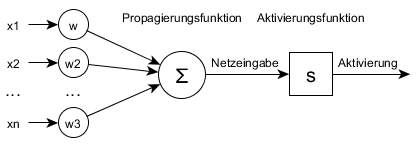
\includegraphics[scale=1.0]{images/neuron.png}
	\caption{Verarbeitung eines Signales in einem Neuron (ohne Ausgabefunktion) (Grafik überarbeiten)}
	\label{img:neuron}
\end{figure}

Wurde ein neuronales Netz konstruiert, folgt darauf die Trainingsphase. Durch das Training ist es möglich, dass ein Netzwerk Neuronen oder Verbindungen hinzufügt bzw. entfernt, den Schwellwert für die Aktivierung von Neuronen verändert oder die Gewichte zwischen Neuronen anpasst. Die Fehlerquote $F$ wird als die Summe der quadrierten Differenz zwischen dem angestrebten Ergebnis $r_{i}$ und der Ausgabe des Netzes $z_{i}$ berechnet:
$$ F()=\sum_{i=1}^{n} (r_{i} - z_{i})^2 $$
Um diese Veränderungen im Netz bekannt zu machen, wird das \textit{Backpropagation} Verfahren genutzt. \textit{Backpropagation} minimiert den Gradientenabstieg auf der Fehleroberfläche die $F$ aufspannt. Der Algorithmus geht in drei Schritten vor:

\begin{enumerate}
	\item \textbf{Forward Pass} Die Gewichte des Netzwerks werden initialisiert und eine Eingabe durch das Netz propagiert. Als Resultat liegt die Ausgabe $z_{i}$ für $i=1,...,n$ vor.
	\item \textbf{Berechnung} Die Summe der quadrierten Fehler $F$ wird berechnet.
	\item \textbf{Backward Pass} In diesem Schritt wird die Fehlerquote rückwärts durch das Netz propagiert. Die Gewichte an den Verbindungen zwischen Neuronen werden in Abhängigkeit ihres Einflusses auf den Fehler aktualisiert.
\end{enumerate}

\begin{itemize}
	\item TODO: Gradienten erläutern
	\item Die Formel für die Fehlerquote wahrscheinlich einfach entfernen oder sollte es hier stattdessen tiefer behandelt werden (Abbildung einer Fläche erzeugt durch F)?
\end{itemize}

\subsection{Funktionsweise}
Ein Autoencoder (AE) ist ein spezielles neuronales Netzwerk, dass eine komprimierte Kodierung der Eingabe lernt. Ein Autoencoder versucht die Daten zu rekonstruieren und kann daher unbeaufsichtigt lernen: Die rekonstruierten Daten können anhand einer Distanzmetrik mit den Originaldaten verglichen werden. Anschließend kann die Größe des Fehlers berechnet werden und durch \textit{Backpropagation} die Gewichtesmatrix aktualisiert werden.
Um die Originaldaten als Ergebnis erhalten zu können, muss die Anzahl der Neuronen des \textit{Input layers} der Anzahl der Neuronen im \textit{Output layer} entsprechen. Die Anzahl der Neuronen im \textit{Hiddenlayer} ist geringer, um die komprimierte Darstellung des Features zu erreichen. Werden mehrere \textit{Hiddenlayer} verwendet, so nimmt die Neuronenanzahl von Layer zu Layer ab um die Anzahl der Dimensionen weiter zu verringern. Dieser Vorgang ist die Enkodierung und liefert die gewünschte komprimierte Abbildung. Die Dekodierung ist umgekehrt aufgebaut, um das Original aus der komprimierten Repräsentation Schicht für Schicht zu rekonstruieren. Wie gut die Dekodierung gelungen ist, lässt sich dann anhand eines Vergleichs der Distanz des Original und der Rekonstruktion bewerten. Formal wird ein Eingabevektor $x \in [0,1]^n$ auf einen Vektor $y \in [0,1]^p$ durch $y = encode_{W,b}(x) = s(Wx + b)$ abgebildet. $W$ ist die Gewichtsmatrix $n \times p$ und $b$ der Bias-Vektor. Diese Parameter werden durch den Autoencoder optimiert. Die Rekonstruktion erfolgt durch die Dekodierungsfunktion: $z \in [0, 1]^n$ wird dann durch $z = decode_{W', b'}(y) = s(W'y + b')$ \cite{ssn1997}.

\begin{enumerate}
	\item TODO: Vorteile eines Autoencoders gegenüber anderen Verfahren (supervised, pretraining)
	\item TODO: Beispiel einbeziehen (\ref{img:example_ae})
	\item Weniger Mathematik oder anhand von Grafik mehr einbeziehen?
\end{enumerate}

\begin{figure}
	\centering

	\begin{tikzpicture}[shorten >=1pt,->,draw=black!50, node distance=\layersep]
    \tikzstyle{every pin edge}=[<-,shorten <=1pt]
    \tikzstyle{neuron}=[circle,fill=black!25,minimum size=17pt,inner sep=0pt]
    \tikzstyle{input neuron}=[neuron, fill=green!50];
    \tikzstyle{output neuron}=[neuron, fill=red!50];
    \tikzstyle{hidden neuron}=[neuron, fill=blue!50];
    \tikzstyle{annot} = [text width=6em, text centered]

    % Draw the input layer nodes
    \foreach \name / \y in {1,...,5}
        \node[input neuron, pin=left:$x_{\y}$] (I-\name) at (0,-\y) {};

    % Draw the hidden layer nodes
    \foreach \name / \y in {1,2,3}
        \path[yshift=-1.0cm]
            node[hidden neuron] (H-\name) at (\layersep,-\y cm) {};
    
    % Draw the output layer nodes
    \foreach \name / \y in {1,...,5}
        \node[output neuron,pin={[pin edge={->}]right:$z_{\y}$}, right of=H-3] (O-\name) at (\layersep,-\y) {};

    % Connect every node in the input layer with every node in the
    % hidden layer.
    \foreach \source in {1,...,5}
        \foreach \dest in {1,2,3}
            \path (I-\source) edge (H-\dest);

    % Connect every node in the hidden layer with the output layer
    \foreach \source in {1,2,3}
        \foreach \dest in {1,...,5}
        	\path (H-\source) edge (O-\dest);

    % Annotate the layers
    \node[annot,above of=H-1, node distance=2.0cm] (hl) {Hidden layer};
    \node[annot,left of=hl] {Input layer};
    \node[annot,right of=hl] {Output layer};
	\end{tikzpicture}

	\caption{Beispiel eines simplen Autoencoders}
	\label{img:example_ae}
\end{figure}

\subsection{Stacked Denoising Autoencoder}

Von Hinton and Salakhutdinov wurde 2006 das Konzept des Stacked Autoencoders eingeführt, um einige Probleme mit herkömmlichen Autoencoder zu überwinden. Bei Netzwerken mit mehr als einem Hidden Layer erzielt die Gradient Descent Methode bei der Rückpropagierung keine guten Ergebnisse mehr, aufgrund der Verzerrung er Gradienten. In vielen Ansätzen wurde auch eine zufällige Initialisierung der Gewichte gewählt. Hier besteht die Gefahr, dass der Algorithmus in einem lokalen Optimum verbleibt. Wenn die anfänglichen Gewichte hingegen bereits nah an einer guten Lösung liegen, sinkt die Wahrscheinlichkeit eines lokalen Optimums. Aus diesem Grund wurde das Pretraining für Autoencoder mit mehr als einer Schicht vorgeschlagen. Das Pretraining besteht aus zwei Schritten, von denen Schritt zwei und drei wiederholt werden, bis alle Gewichte trainiert sind.

\begin{enumerate}
	\item Es wird der unterste Autoencoder zuerst trainiert. Also der Autoencoder der aus dem \textit{Input-} und folgendem \textit{Hidden layer} besteht.
	\item Nun wird der Decoder des trainierten Autoencoders entfernt und ein neuen Autoencoder erzeugt. Dieser besitzt den \textit{Hidden layer} des trainierten Autoencoders als \textit{Input layer}.
	\item Das Training wird mit dem neuen Autoencoder fortgeführt.
\end{enumerate}

\cite{sda2010}

\begin{itemize}
	\item TODO: Abbildungen
	\item TODO: Denoising Autoencoder
\end{itemize}

\section{GPGPU Programmierung}

Der Begriff General Programming on Graphics Processing Units (GPGPU) beschreibt das Verwenden von Grafikkarten für Berechnungen, die nicht mit der Verarbeitung von grafischen Daten in Zusammenhang stehen. Zur Ausführung wird das Single Program Multiple Data (SPMD) Modell verwendet. Dies bedeutet, dass alle Prozessoren das gleiche Programm auf unterschiedliche Daten anwenden. Da Grafikkarten eine große Anzahl von Kernen enthalten, eignen sie sich sehr gut für die Parallelisierung von Algorithmen. In den letzten Jahren konnten so enorme Steigerungen der Gleitkommaoperationen pro Sekunde (flops) und der Speicherbandbreite erzielt werden. 

\subsection{Nvidia cuda}

Ein Programm, dass auf einer Nvidia Grafikkarte ausgeführt werden soll, muss in der cuda Sprache geschrieben sein. Hierbei handelt es sich um eine Erweiterung von C um primitive und Funktionen für Berechnungen auf der Grafikkarte. Zum Übersetzen und Linken des Codes dient der \textit{nvcc} Compiler von Nvidia. Dieser unterscheidet zwischen Code der auf dem \textit{host}, der CPU, und dem \textit{device}, der GPU, ausgeführt wird. Das Kompilieren von \textit{host} Code erfolgt durch den auf dem \textit{host} installierten C Compiler. Der \textit{device} Code wird durch \textit{nvcc} zu PTX bzw. cubin binary code übersetzt.
Nvidia hat das SPMD Modell durch \textit{kernels} umgesetzt. Ein \textit{kernel} ist ein Programm, dass parallel auf verschiedene Daten der GPU angewendet wird. Um kenntlich zu machen, dass es sich um Code handelt der vom \textit{host} aufgerufen und auf der Grafikkarte ausgeführt wird, muss eine Funktion mit \textit{\_\_global\_\_} spezifiziert werden.
Bevor ein \textit{kernel} aufgerufen werden kann, muss der notwendige Speicher auf der Grafikkarte für die Daten und das Ergebnis allokiert werden. Anschließend werden die Daten von \textit{host} zu \textit{Device} kopiert. Nach Durchführung der Berechnung kann dann das Ergebnis zurück zum \textit{host} kopiert werden. Die Datentransfers weisen eine nicht unbeachtliche Latenz auf. Folglich sollte das Kopieren von Daten nur selten erfolgen.
Die Daten liegen in der Regel als Vektor oder Matrix vor. Der Zugriff auf verschiedene Elemente durch unterschiedliche \textit{kernel} erfolgt dann durch eine Indexberechnung.
Um die Indexberechnung nachvollziehen zu können, muss zunächst die Organisierung von Threads in einem \textit{kernel} näher betrachtet werden. TODO

\begin{figure}
	\centering
	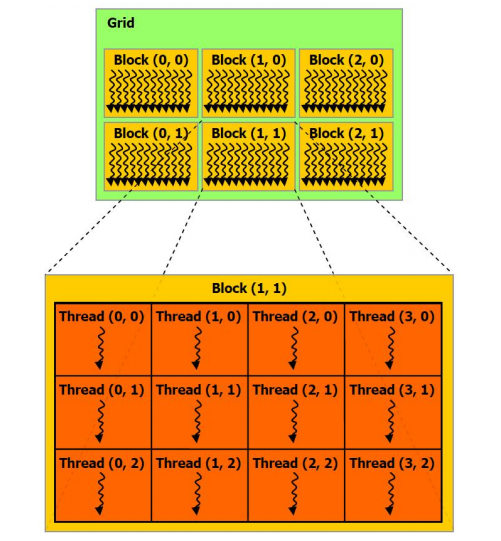
\includegraphics[scale=0.55]{images/cuda1.png}
	\caption{Organisierung von Threads in Blocks in Grids REF}
	\label{img:cuda1}
\end{figure}

\begin{itemize}
	\item TODO: Machine Learning im Intro unterbringen
	\item TODO: Organisierung Grids, Blocks, Threads
	\item TODO: Beispiel anhand von Vektor / Matrix
	\item shared memory ?
\end{itemize}

\subsection{Histogramme parallel berechnen}

Ein häufig eingesetztes Muster, da es sich hervorragend für parallele Berechnungen eignet, ist das Histogramm. Hierbei wird die Häufigkeit einer Wertmenge in Klassen eingeteilt. Histogramme finden Anwendung bei der Extraktion von Features und TODO. Eine große Menge Features kann so in k Klassen eingeteilt werden, der Anzahl oder Größe vorgegeben werden kann. Pro Feature wird die entsprechende Klasse um eins inkrementiert. Dies kann parallel durchgeführt werden da die Operation assoziativ und kommutativ ist: Es spielt keine Rolle in welcher Reihenfolge die Features abgearbeitet werden. Wenn das zu beschreibende Histogramm im global Speicher vorliegt, wird die Berechnungsgeschwindigkeit stark reduziert, da viele Threads auf die gleichen Speicheradressen des Histogramms schreibend zugreifen. Damit keine Dies wird in cuda durch die Operation \textit{atomicAdd} Um dies zu umgehen, wird pro Block in einem Grid eine lokales, privates Histogramm im shared Memory angelegt. Dadurch müssen aber noch die Werte der privaten Histogramme in das globale kumuliert werden, sobald alle Threads eines Blocks fertig sind.

\lstset{language=C}
\begin{lstlisting}
__global__
void histogram_kernel (float *buffer, long size, int *histo) {
	__shared__ int *copy[10];
	
	if (threadIdx.x < 10) {
		copy[threadIdx.x] = 0;		
	}
	__syncthreads();

	int id = threadIdx.x + blockDim.x * gridDim.x;
	int stride = blockDim.x * gridDim.x;
	
	while (i < stride) {
		int bin = buffer[i] / 10; 
		atomicAdd(&(copy[bin]), 1);
		i += stride;	
	}
	__syncthreads();
	
	if (threadIdx.x < 10) {
		atomicAdd(&(histo[threadIdx.x]), copy[threadIdx.x]);		
	}
}
\end{lstlisting} 

\begin{itemize}
	\item Histogramm verschieben nach Analyse / Konzept?
\end{itemize}
\chapter{Analyse}

Ziel dieser Arbeit ist es ein Modell zu entwickeln, dass es ermöglicht große Mengen von Bildern zu gruppieren. Durch die großen Mengen an Daten die zu verarbeiten sind, sollen \textit{state of the art} Verfahren genutzt werden, die speziell hierauf ausgelegt sind. Der erste der Teil der Analyse befasst sich daher mit dem Bereich des \textit{Machine Learning}. Hier handelt es sich um keine umfängliche Einführung. Es werden Methoden beleuchtet, die zur Komprimierung und Gruppierung von Daten dienen und die Basis des hier vorgeschlagenen Modells bilden. Anhand der Anforderungen und Annahmen wird dann ein unüberwachtes Lernverfahren ausgewählt, dass zu Gruppierung von Bildern dient und in den folgenden Kapiteln weiter ausgearbeitet und realisiert wird. \newline
Im zweiten Teil sollen Möglichkeiten untersucht werden, aus Bildern Features zu gewinnen, welche als Eingabe für das Modell dienen. Um einen Überblick über Features in der Bildverarbeitung zu gewinnen, werden zunächst einige Feature-Detektoren bzw. Deskriptoren für unterschiedlicher Anwendungsfälle angeführt. Heute ist es kaum vorstellbar, dass ein Feature-Deskriptor jeden möglichen Anwendungsfall abdecken kann. Daher soll abschließend der Fokus dieser Arbeit festgelegt werden: Sollen beispielsweise Gesichter oder Szenen erkannt werden? Sollen Objekte erkannt werden und wenn ja, beliebige Kategorien? Anhand der gewonnen Erkenntnisse wird dann entschieden, welche Eigenschaften der hier verwendete Feature-Deskriptor aufweisen soll. 

\section{Verwendung der GPU}

Zum Aufbauen eines Modells werden mehrere Zehn- bis Hunderttausend Features verarbeitet werden. Viele der Verfahren, die der Erzeugung solcher Modellen zu Grunde liegen, wurden in den vergangenen Jahren durch die Verwendung der GPU statt der CPU beschleunigt. Bei der Betrachtung geeigneter Ansätze wird daher auch berücksichtigt, ob und wie eine Beschleunigung durch parallele Verarbeitung erzielt werden kann. Gerade bei großen Datenmengen und einer enormen Datenparallelität können Probleme durch GPUs um ein vielfaches schneller gelöst werden als durch CPUs. Da Nvidias CUDA an der Hochschule Hannover sowohl gelehrt als auch zu Forschungszwecken genutzt wird und sich CUDA auch international in Forschung und Wirtschaft etabliert hat, soll die Plattform als technische Basis dienen. 

\section{Machine Learning}

\textit{Machine Learning} ist ein Teilgebiet der künstlichen Intelligenz und wird genutzt um System zu entwerfen, die nicht explizit programmiert werden. Stattdessen Lernen diese Systeme: Lernen bedeutet in diesem Kontext, dass eine System durch eine Eingabe seine Struktur verändert, um so die erwartete Leistung zu steigern. Dabei ist \textit{Machine Learning} ein interdisziplinäres Feld: Es sind sowohl Computerwissenschaften, Statistik als auch biologische und kognitive Wissenschaften involviert. Bisher haben sich viele Anwendungsfälle für \textit{Machine Learning} Verfahren ergeben, die bis in den Alltag reichen. Einige Beispiele sind:

\begin{itemize}
	\item \textbf{Optical Character Recognition (OCR)} Unter OCR wird das Übersetzen eines (hand-)geschriebenen Textes in eine digitales Dokument bezeichnet. Beispielsweise kann so das Einfügen von Daten in CRM / ERP System automatisiert werden.
	\item \textbf{Spam Filterung} Das automatische Erkennen von unerwünschten E-Mails, die Werbung enthalten oder Betrugsversuche sind, ist inzwischen bei jedem Mail-Anbieter Teil des Angebots.
	\item \textbf{Spracherkennung} Auch eine Spracherkennung ist bereits auf den meisten digitalen Assistenten verfügbar und wird sogar zur Steuerung der häuslichen Elektronik verwendet.
	\item \textbf{Anomalie Erkennung} Digitale Geldtransaktionen werden heute von Algorithmen überwacht, die Abweichungen im Zahlungsverhalten beobachten. Wird eine ungewöhnlich hohe Summe überwiesen oder abgehoben, kann so informiert und auch interveniert werden.
\end{itemize}

All diese Verfahren nutzen eine große Menge an Trainingsdaten, um so ein Modell zu generieren, welches eine Klassifizierung weiterer Daten ermöglicht. Beispielsweise müssen bei einem System zur Spam-Filterung sowohl \enquote{normale} als auch Spam E-Mails verwendet werden, eine Spracherkennung benötigt digitale Aufnahmen von Wörtern und Sätzen zum Lernen, etc.
Nach dem Aufbau des Modells findet dann durch das System die Klassifizierung von Test- bzw. realen Daten statt. Es wird beispielsweise bei OCR entschieden, welches digitale Pendant zum vorliegenden Zeichen gehört oder bei der Spam-Filterung wie hoch die Wahrscheinlichkeit ist, dass es sich bei einer Mail um Spam handelt. Diese Trainings- und Testphase sind typisch für \textit{Machine Learning} Ansätze. Allgemein eignet sich dieser Ansatz:

\begin{itemize}
	\item Um Beziehungen und Muster in den Daten zu entdecken, die nicht offensichtlich sind. Genau mit dieser Fragestellung beschäftigt sich die Disziplin des \textit{Data Mining}. Hierfür werden u.a. maschinelle Lernalgorithmen genutzt.
	\item Wenn kein klassischer Algorithmus für die Problemstellung entworfen werden kann oder das Programm zu komplex ist, als das es von Menschen kodiert und gewartet werden könnte.
	\item Um neue Informationen einzubeziehen. Das Modell basiert auf den Daten, daher kann das System sich theoretisch durch neue Daten verändern und so der Situation anpassen.
\end{itemize}

\subsection{Lernverfahren}

Je nach Fragestellung haben sich unterschiedliche Methodiken entwickelt, um den Lernprozess in einem System abzubilden. Im Wesentlichen werden drei Arten des maschinellen Lernens unterschieden:

\begin{itemize}
	\item \textbf{Überwachtes Lernen (supervised learning)} Ein überwachtes Lernverfahren soll eine Funktion $f$ lernen, die Eingaben ($x$) ihren Ausgaben ($y$) zuordnet, sodass gilt: $y = f(x)$ . Diese Funktion wird anhand von Trainingsdaten gelernt, die demzufolge aus Paaren von Eingaben und ihren dazugehörigen Ausgaben bestehen.
	\item \textbf{Unüberwachtes Lernen (unsupervised learning)} Ziel unüberwachter Lernalgorithmen ist es, großen Mengen von nicht kategorisierten Daten zu gruppieren oder zu komprimieren. Dadurch können Beziehungen in den Daten entdeckt bzw. kompaktere Darstellungen erreicht werden.
	\item \textbf{Verstärkendes Lernen (reinforcement learning)} Beim verstärkenden Lernen hat ein Agent die Aufgabe ein vorgegebenes Ziel zu erreichen, indem er mit seiner Umwelt agiert. Die Umwelt ist dabei eine Menge von Zuständen zwischen denen der Agent durch eine Aktion wechselt. Dabei hat jede Aktion eine Belohnungen oder Bestrafungen zufolge. Der Agent optimiert dann sein Verhalten, um die erhaltenen Belohnungen zu maximieren.
\end{itemize}

Beim überwachten Lernen ist es notwendig, dass sowohl Ursachen (Eingaben) als auch Effekte (Ausgaben) gemessen wurden. Hier sollen dann durch ein trainiertes Modell eine Vorhersage der Ausgabe abhängig von der Eingabe erfolgen. Beim unüberwachten Lernen hingegen sind die Eingaben latente Variablen. Das heißt sie sind nicht direkt gemessen worden, sondern durch mathematische Verfahren von Observationen abgeleitet. Dadurch ist ein exploratives Vorgehen möglich. Es können Beziehungen in den Daten entdeckt und Gruppierungen bzw. Klassifizierungen durchgeführt werden.

\subsection{Unüberwachte Lernverfahren im Kontext dieser Arbeit}

Für die Gruppierung des Bildmaterials eignen sich maschinelle Lernverfahren besonders, da sie zum einen auf eine große Menge an Trainingsdaten angewiesen sind, um ein nützliches Modell zu generieren und zum anderen eine parallele Verarbeitung begünstigen. In dieser Arbeit werden hierfür unüberwachte Lernverfahren aus folgenden Gründen genutzt:

\begin{itemize}
	\item Das Gruppieren bzw. Kategorisieren von Daten (\textit{Clustering}) ist selbst ein Teilgebiet innerhalb der unüberwachten Lernverfahren.
	\item Die Feature-Vektoren umfassen oft viele Komponenten, welche zur Kodierung der Eigenschaften erforderlich sind. Im Bereich des \textit{Machine Learning} gibt es Verfahren, welche die Feature-Vektoren auf ihre wesentlichen Komponenten analysieren und so eine kompaktere Darstellung erzeugen.
	\item Es sollen Darstellungen bzw. Strukturen in den Daten entdeckt werden, die nicht a priori bekannt sind. Ein überwachter Ansatz erfordert zum Training \textit{gelabelte} Daten, um Vorhersagen zu treffen. Da die gesuchten Strukturen aber gerade nicht bekannt sind, scheidet ein überwachter Ansatz aus.
\end{itemize}

Hieraus geht hervor, dass zum Gruppieren der Bild-Features ein \textit{Clustering} Verfahren notwendig ist. Diese Art von Algorithmen und einige ihrer Vertreter werden daher im Folgenden vorgestellt. Außerdem scheint es sinnvoll die Features vor dem Clustering aufzubereiten: Durch eine kompaktere Darstellung der Feature-Vektoren kann der notwendige Speicher reduziert und die Berechnung beschleunigt werden. Nach dem Clustering folgt daher einer Übersicht über den Bereich \textit{Dimensionality Reduction (Reduzierung der Dimensionalität}: Diese Art von Algorithmen hat die Kompression von Daten zum Ziel.

\textbf{Clustering-Verfahren} quantisieren die Daten in Gruppen. Eine Gruppe steht hier für ein semantisches Merkmal und vertritt eine Menge von konkreten Daten. Unter Clustering Verfahren fallen Algorithmen wie k-means, hierarchical clustering oder etwa das Gaussian Mixture Model.\newline
Ein Clustering Algorithmus hat in dem Kontext dieser Arbeit das Ziel, eine großen Menge Feature-Deskriptoren auf die Wesentlichen zu reduzieren. Durch diese Quantisierung in $n$ Gruppen müssen, bei einer Bewertung eines neuen Deskriptors, nur Vergleiche mit $n$ Deskriptoren durchgeführt werden, statt mit jedem Deskriptor der Ursprungsmenge.\newline

\textbf{Verfahren zu Reduzierung der Dimensionalität} nehmen an, dass es eine unterliegende Struktur gibt, welche entdeckt werden kann. In diesem Fall vertreten die Dimensionen semantische Merkmale. Methoden wie beispielsweise die Hauptkomponentenanalyse bilden die Feature-Vektoren auf einen Raum niederer Dimensionen ab. \newline
Ein moderneren Ansatz für diesen Zweck ist die Verwendung neuronaler Netze. Ein Autoencoder ist ein spezielles neuronales Netzwerk, welches für das Lernen einer komprimierten Darstellung von Daten verwendet wird. Das Konzept des Autoencoders reicht zwar bis in 80er Jahre zurück, eine Methode zum Training tiefer Netze ist aber erst 2006 von Hinton entwickelt worden.\newline

Um einen kompakteren Feature-Deskriptor zu erzeugen soll ein Autoencoder verwendet werden. Ein mehrstufiger Autoencoder kann mit jeder Schicht einen kompakteren Deskriptor erzeugen und kodiert die gelernten Informationen in den Gewichten. Der Autoencoder bringt darüber hinaus den Vorteil mit sich, das seine Architektur bereits auf eine parallele Verarbeitung ausgelegt ist und nicht \enquote{extra} berücksichtigt werden muss. Des Weiteren sind klassische Methoden wie die Hauptkomponentenanaylse bereits zahlreich betrachtet worden. Ein Autoencoder hingegen ist in diesem Bereich, im Vergleich, ein neuer Vertreter, dessen vielfältige Einsatzmöglichkeiten immer noch erforscht werden. \todo{Vorteile Autoencoder}. \newline  
Um die Features zu Gruppieren soll ein k-means Clustering Verfahren verwendet werden. Anhand der durch k-means gewonnen Cluster kann eine Histogrammdarstellung für Features erzeugt werden. Die Kombination diese Verfahren wird Bag of Visual Words genannt und lehnt sich an das Bag of Words Modell an. Hinsichtlich der Berechnung durch eine GPU, sind diese Verfahren auch gut geeignet: Die Familie der k-means Algorithmen enthält viele Algorithmen die lange etabliert sind und bereits für die parallele Ausführung auf Grafikkarten adaptiert wurden. Das parallele Verarbeiten von Histogrammen ist ein Lehrbuchbeispiel für den Einsatz von Grafikkarten, da es durch parallelen Reduzierung, ein Muster für einige Probleme, erreicht werden kann.

\section{Autoencoder}

Durch den Aufschwung des maschinellen Lernens in den letzten Jahren sind neuronale Netze stark in den Fokus der Industrie und Wissenschaft gerückt. Solche künstlichen neuronalen Netze werden genutzt, um aus Beispielen Muster zu lernen und diesen Wissen zu transferieren. 
Ein spezielles neuronales Netzwerk zum unbeaufsichtigten Lernen ist der Autoencoder. Diese Art von Netzwerk lernt selbstständig eine komprimierte Darstellung der Eingabe. 
Als erstes wird im folgenden Abschnitt der Aufbau und die Funktionsweise eines Autoencoders erläutert. Darauf aufbauend werden zwei Erweiterungen des Autoencoders vorgestellt: Der Stacked Autoencoder und der Denoising Autoencoder. Ersterer wird verwendet, um effektiv tiefe Netzwerke zu konstruieren, letzterer ermöglicht eine korrekte Konstruktion aus verzerrten Daten.

\subsection{Aufbau und Funktionsweise}

Ein Autoencoder (AE) ist ein spezielles neuronales Netzwerk, dass eine komprimierte Kodierung der Eingabe lernt. Ein Autoencoder versucht die Daten zu rekonstruieren und kann daher unbeaufsichtigt lernen: Die rekonstruierten Daten können anhand einer Distanzmetrik mit den Originaldaten verglichen werden. Anschließend kann die Größe des Fehlers berechnet werden und durch \textit{Backpropagation} die Gewichtesmatrix aktualisiert werden \cite{ssn1997}.
Um die Originaldaten als Ergebnis erhalten zu können, muss die Anzahl der Neuronen des \textit{Input Layers} der Anzahl der Neuronen im \textit{Output Layer} entsprechen. Die Anzahl der Neuronen im \textit{Hidden Layer} ist geringer, um die komprimierte Darstellung des Features zu erreichen. Werden mehrere \textit{Hidden Layer} verwendet, so nimmt die Neuronenanzahl von Schicht zu Schicht ab um die Anzahl der Komponenten weiter zu verringern. Dieser Vorgang ist die Enkodierung und liefert die gewünschte komprimierte Abbildung. Die Dekodierung ist umgekehrt aufgebaut, um das Original aus der komprimierten Repräsentation Schicht für Schicht zu rekonstruieren. Wie gut die Dekodierung gelungen ist, lässt sich dann anhand eines Vergleichs der Distanz des Original und der Rekonstruktion bewerten.\newline
Formal wird ein Eingabevektor $x \in [0,1]^n$ auf einen Vektor $y \in [0,1]^p$, mit $p < n$, abgebildet: 
$$y = encode_{W,b}(x) = s(Wx + b)$$
$W$ ist die Gewichtsmatrix der Größe $n \times p$ und $b$ der Bias-Vektor. Diese Parameter werden durch den Autoencoder optimiert. Die Darstellung $y$ wird in diesm Kontext auch als \textit{code} bzw. latente Variablen bezeichnet. Die Rekonstruktion erfolgt durch die Dekodierungsfunktion. Der Vektor $z \in [0, 1]^n$ berechnet sich durch: 
$$z = decode_{W', b'}(y) = s(W'y + b')$$
In Abbildung \ref{img:example_ae} ist ein Autoencoder abgebildet der als Eingabe einen Vektor $x \in [0,1]^4$ entgegen nimmt. Dieser wird auf den Vektor $y$ mit drei Komponenten abbildet, da der \textit{Hidden Layer} drei Neuronen enthält. Die Rekonstruktion $z$ aus $y$ erfolgt dann durch die Berechnung der Dekodierungsfunktion.

\begin{figure}
	\centering

	\begin{tikzpicture}[shorten >=1pt,->,draw=black!50, node distance=\layersep]
    \tikzstyle{every pin edge}=[<-,shorten <=1pt]
    \tikzstyle{neuron}=[circle,fill=black!25,minimum size=17pt,inner sep=0pt]
    \tikzstyle{input neuron}=[neuron, fill=green!50];
    \tikzstyle{output neuron}=[neuron, fill=red!50];
    \tikzstyle{hidden neuron}=[neuron, fill=blue!50];
    \tikzstyle{annot} = [text width=6em, text centered]

    % Draw the input layer nodes
    \foreach \name / \y in {1,...,4}
        \node[input neuron, pin=left:$x_{\y}$] (I-\name) at (0,-\y) {};

    % Draw the hidden layer nodes
    \foreach \name / \y in {1,2,3}
        \path[yshift=-0.5cm]
            node[hidden neuron] (H-\name) at (\layersep,-\y cm) {$y_{\y}$};
    
    % Draw the output layer nodes
    \foreach \name / \y in {1,...,4}
        \node[output neuron,pin={[pin edge={->}]right:$z_{\y}$}, right of=H-3] (O-\name) at (\layersep,-\y) {};

    % Connect every node in the input layer with every node in the
    % hidden layer.
    \foreach \source in {1,...,4}
        \foreach \dest in {1,2,3}
            \path (I-\source) edge (H-\dest);

    % Connect every node in the hidden layer with the output layer
    \foreach \source in {1,2,3}
        \foreach \dest in {1,...,4}
        	\path (H-\source) edge (O-\dest);

    % Annotate the layers
    \node[annot,above of=H-1, node distance=1.5cm] (hl) {Hidden Layer};
    \node[annot,left of=hl] {Input Layer};
    \node[annot,right of=hl] {Output Layer};
	\end{tikzpicture}

	\caption{Beispiel eines simplen Autoencoders}
	\label{img:example_ae}
\end{figure}

\subsection{Stacked Denoising Autoencoder}

Von Hinton and Salakhutdinov wurde 2006 das Konzept des Stacked Autoencoders eingeführt, um einige Probleme mit herkömmlichen Autoencoder zu überwinden \cite{dae2006}. Bei Netzwerken mit mehr als einem \textit{Hidden Layer} erzielt die Gradientenabstiegs-Methode, aufgrund der zunehmenden Verzerrung der Gradienten, bei der Rückpropagierung keine guten Ergebnisse mehr. In vielen Ansätzen wurde auch eine zufällige Initialisierung der Gewichte gewählt. Hier besteht die Gefahr, dass der Algorithmus in einem lokalen Optimum verbleibt. Wenn die anfänglichen Gewichte hingegen bereits nah an einer guten Lösung liegen, sinkt die Wahrscheinlichkeit eines lokalen Optimums. Aus diesem Grund wurde das Pretraining für Autoencoder mit mehr als einer Schicht vorgeschlagen. In diesem Training wird jedes Paar aneinanderliegender Schichten als ein Autoencoder aufgefasst und einzeln trainiert. Das Pretraining besteht aus drei Schritten, die wiederholt werden, bis alle Autoencoder trainiert sind.

\begin{enumerate}
	\item Es wird der aktuelle Autoencoder trainiert. Zu Beginn besteht dieser aus dem \textit{Input} und folgendem \textit{Hidden Layer}.
	\item Nun wird der Decoder des trainierten Autoencoders entfernt und ein neuer Autoencoder erzeugt. Dieser besitzt den \textit{Hidden Layer} des trainierten Autoencoders als \textit{Input Layer}.
	\item Das Training wird mit dem neuen Autoencoder fortgeführt.
\end{enumerate}

Ein Denoising Autoencoder \cite{sda2010} dient dazu, eine korrumpierte Eingabe zu korrigieren. Die Korruption ist hier als Rauschen bzw. Verzerrung (\textit{noise}) aufzufassen. In vielen Arten von Features, z.B. Bildern oder Audiomaterial, sind Verzerrungen bereits in den Daten vorhanden, beeinflussen die Semantik des Ganzen aber kaum. Daher soll der Autoencoder dies bereits berücksichtigen, indem er nicht direkt mir der Eingabe $x$ arbeitet. Stattdessen wird $x$ auf die korrumpierte Eingabe $\widetilde{x}$ durch ein stochastisches Verfahren abgebildet. In der Enkodierungsfunktion wird dann $\widetilde{x}$ statt $x$ verwendet: 
$$encode_{W,b}(\widetilde{x}) = s(W\widetilde{x} + b)$$
In der Praxis hat sich zur Korruption der Eingabe die \textit{masking corruption} Technik bewährt: Hierbei werden 20\% bis 50\% der Neuronen des \textit{Input Layers} zufällige ausgewählt und werden \enquote{genullt}. Auf diese Weise wird vermieden, dass der Autoencoder nur von bestimmten Teilmengen an Neuronen abhängt  \cite{pda2012}.

\subsection{Hyperparameter}

Bisher wurde das Netzwerk und die Parameter die es optimiert, die Gewichte $w$ und der Bias-Vektor $b$, betrachtet. Darüber hinaus gibt es eine Reihe von Parametern, die Hyperparameter, die vor Anwendung des Modells festgelegt werden müssen. Die wesentlichen Hyperparameter für neuronale Netze sollen hier vorgestellt und ihr Einfluss auf das Modell erläutert werden. Die aufgeführten Standardwerte wurden bei einer Vielzahl von Modellen beobachtet, gelten aber nicht uneingeschränkt für jeden Anwendungsfall \cite{pda2012}. 
%https://arxiv.org/pdf/1206.5533.pdf

\begin{itemize}
	\item \textbf{Initiale Lernrate} Bei gradientenbasierten Vefahren wird in jeder Iteration der Fehler zurückpropagiert. Dies wird in den meisten Fällen zu einer zu schnellen Anpassung des Netzes führen und es \enquote{vergisst} schnell, was es bereits gelernt hat. Aus diesem Grund werden die berechneten Fehler mit der Lernrate (\textit{learning rate}), einem kleinen Wert, multipliziert. Praktisch wird für die Lernrate ein Wert kleiner 1 und größer $10^{-6}$ verwendet.
	\item \textbf{Anzahl der Trainingsiteration} Eine Iteration entspricht einem \textit{forward} und \textit{backward pass} einer kleinen Teilmenge (ein \textit{batch}) der gesamten Trainingsmenge. Eine zu große Anzahl an Iterationen führt zu einer Überanpassung des Netzes an die Trainingsdaten, daher sollte gestoppt werden, wenn sich andere Metriken nicht mehr verbessern.
	\item \textbf{Anzahl der Exemplare pro Trainingsiteration} (\textit{batch size)} Je größer die \textit{batch size}, desto mehr Trainingsexemplare werden pro Iteration verarbeitet. Durch einen größeren Wert kann die Berechnung beschleunigt werden, allerdings ist auch mehr Speicher erforderlich. In der Praxis liegt der Wert für diesen Parameter meist zwischen 16 und 128 (Zweierpotenzen). 
\end{itemize}

\section{Bag of Visual Words}

Das Bag of Visual Words lehnt sich an das Bag of Words Modell aus dem Bereich Information Retrival an. Daher soll zunächst die Funktionsweise des Bag of Word Modells erläutert werden, um darauf aufbauend den Bag of Visual Words einzuführen.\newline 
Der Bag of Words wird zur Klassifizierung von Dokumenten genutzt. Beim Bag of Words wird das Auftreten jedes Wortes in einem Dokument gezählt und durch die Anzahl aller Wörter im Vokabular dividiert, um so einen normalisierten Wert zu erhalten, welcher die relative Häufigkeit eines Wortes angibt. Das Vokabular wird \textit{Codebook} genannt, die Wörter werden auch als \textit{Codewords} bezeichnet.\newline
Dieses Modell wurde von der digitalen Bildverarbeitung adaptiert \cite{bok2004}. Es wird anhand der Features von Trainingsbildern ein visuelles Vokabular gelernt, das zur Klassifizierung von Bildern dient. Die Features können aber nicht direkt statt der Worthäufigkeit verwendet werden: Ein Wort ist ein diskreter Wert der direkt verglichen werden kann, ein Feature hingegen ist ein Vektor in einem hochdimensionalen Raum, der Eigenschaften beschreibt. Um konkrete Werte zu erhalten, ist es notwendig, die Vektoren zu quantisieren. Die quantisierten Vektoren entsprechen dann den \textit{Codewords} und werden in diesem Kontext auch \textit{Visual Words} genannt. \newline
Zunächst wird die Funktionsweise des Bag of Visual Words im folgenden Abschnitt näher betrachtet. Dem schließt eine Betrachtung des Kernstücks des Algorithms an: Das Clustering der Features. Hier wird ein k-means Algorithmus, Llyods heuristische Variante, verwendet. Es wird eine gängige sequentielle Implementierung angeführt, auf deren Basis dann die Parallelisierbarkeit durch Grafikkarten untersucht wird.\newline
Bei der Einordnung eines Bildes wird ein Histogramm der Visual Words generiert, daher wird im Anschluss ein sequentieller Histogramm Algorithmus vorgestellt, der auf Parallelisierbarkeit geprüft wird.

\subsection{Funktionsweise}

Der Bag of Visual Words besteht aus einer Trainings- und Testphase, wie in Abbildung \ref{img:bovw} dargestellt. Die Extraktion der Features ist beiden Phasen vorgelagert.\newline
Zu Beginn erfolgt die Trainingsphase, das Clustering der extrahierten Features. Das so erzeugte \textit{Codebook} ist das Modell, gegen das anschließend getestet werden kann. Die Idee ist, dass ähnliche Feature-Vektoren nah beieinander im Raum liegen und somit in die gleiche semantische Kategorie gehören. Durch einen Clustering Algorithmus wie k-means kann die Größe des \textit{Codebooks} bestimmt werden. Wird für $k$ ein große Zahl gewählt, wird ein Vokabular von Exemplaren aufgebaut, ein kleines $k$ hingegen erkennt eher Kategorien. Die Schwerpunkte der Cluster vertreten dann eine Menge von ähnlichen Features und bilden das \textit{Codebook} bzw. Modell.\newline
Der Testprozess erzeugt nun, auf Basis des \textit{Codebooks}, die \textit{Visual Words} von Bildern. Hierfür werden die Features eines Bildes extrahiert und ein Histogrammalgorithmus ermittelt die Verteilung der \text{Visual Words}: Für jedes Feature wird das ähnlichste \textit{Visual Word} des \textit{Codebooks} bestimmt und die entsprechende Klasse inkrementiert. Wird dieser Prozess auf zwei Bilder angewendet, so können die resultierenden Histogramme miteinander verglichen werden (z.B. mit dem \textit{MSE (mean squared error)} als Metrik.

\begin{figure}
	\centering
	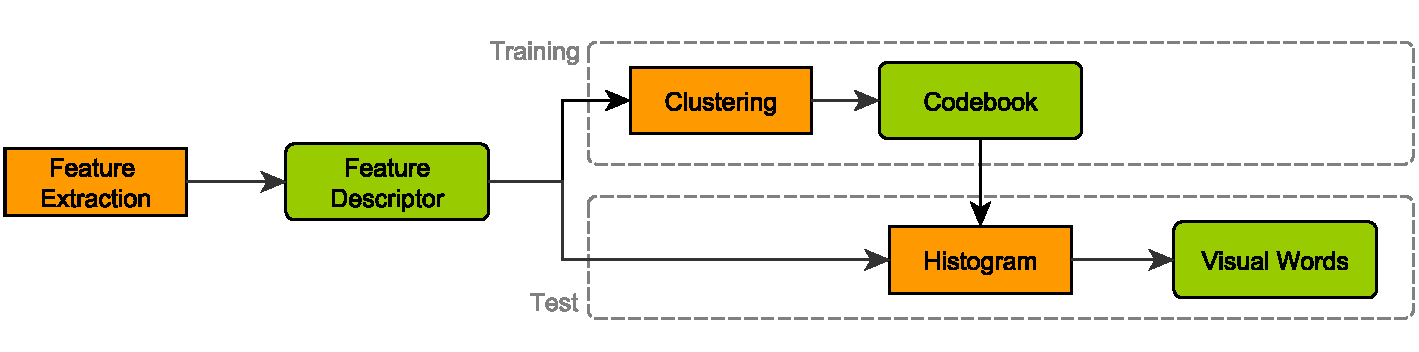
\includegraphics[scale=0.65]{images/bovw_process.pdf}
	\caption{Training- und Testprozess des Bag of Visual Word Modells.}
	\label{img:bovw}
\end{figure}

\subsection{Lloyds Algorithmus}

Im Grundlagenkapitel wurde bereits Lloyds Algorithmus eingeführt, hier soll zunächst näher auf die sequentielle Ausführung eingegangen werden, um anschließend eine mögliche Parallelisierung zu diskutieren. Im nachfolgenden Codelisting ist der Ablauf des Algorithmus in Pseudocode beschrieben. Als Parameter werden die Punkte $P$ und die Anzahl der zu bildenden Cluster $k$ erwartet. In Zeile 2 findet die Auswahl der initialen Schwerpunkte der Cluster statt. Die Zuordnung von Punkten zu Clustern erfolgt in Zeile 7: $argminD$ wählt den Cluster aus, dessen Varianz am Wenigsten bei Aufnahme des Punktes $p_{i}$ steigt. Abschließend wird die Aktualisierung der Schwerpunkte aller Cluster in der Schleife in Zeile 8 und 9 durchgeführt.

\lstset{language=C}
\begin{lstlisting}[mathescape=true]
kmeans_lloyd ($P, C, k$)
	initialisierung
	until convergence
		$C_{j} = 0, j = 1, ..., k$
		for each $p_{i} \in P$
			for each $c_{j} \in C$
				$c_{j} = argminD(c_{j}, p_{i})$		
		for each $c_{j} \in  C$
			$c_{j} = \frac{1}{|c_{j}|} \sum_{n_{i} \in c_{j}} n_{i}$
\end{lstlisting}

Die Initialisierungsphase muss für die Parallelisierung nicht beachtet werden: Sie nimmt nur wenig Zeit in Anspruch und wird einmalig zu Beginn ausgeführt. Die Anderen beiden Schritte des Algorithmus bergen mehr Potential: In Zeile 5 bis 7 wird die Varianz jedes Cluster-Vektor Paares berechnet. Da die Berechnung der Varianz eines Paares unabhängig von der eines anderen ist, kann die Berechnung aller Varianzen parallel erfolgen. Nachdem für einen Durchgang die Veränderung der Mitgliedschaft von Vektoren zu Clustern berechnet wurde, müssen die Cluster-Schwerpunkte aktualisiert werden. Auch die Berechnung der neuen Schwerpunkte der Cluster kann unabhängig voneinander erfolgen: Die Vektoren aus denen der Mittelwert berechnet wird, sind genau einem Cluster zugeordnet.

% http://www.know-center.tugraz.at/download\_extern/papers/latex8.pdf

\subsection{Histogramme}

Ein sequentielles Histogramm kann als Programm in einer Schleife über die Daten ausgedrückt werden: Für jedes Element wird der Index der Klasse des Histogramms berechnet und um eins inkrementiert. Zur Normalisierung des Histogramms ist es anschließend notwendig, jede Klasse des Histogramms durch die Gesamtanzahl der Werte zu dividieren. Da es sich bei der Anzahl der Klassen jedoch um eine kleine Zahl, im Vergleich zur Anzahl der Elemente in den Daten, handelt, ist dieser Aufwand vernachlässigbar.
Um das Histogramm der Visual Words eines Bildes zu erzeugen, muss für jedes extrahierte Feature das nächste Visual Word bestimmt werden. Dies entspricht im nachfolgenden Pseudocode der doppelten Schleife über die Features $F$ und Cluster $C$ in Zeile 2 und 3. Der Index des nächsten Clusters wird dann in Zeile 4 durch $argmin D$ berechnet und in der nächsten Zeile wird das Histogramm $H$ an der entsprechenden Stelle inkrementiert.

\begin{lstlisting}[mathescape=true]
histogram ($P, C, H$)
	for each $p_{i} \in P$
		for each $c_{j} \in C$
			$k = arminD(c_{j}, p_{i})$ 
		$H_{k} = H_{k} + 1$		
	for $1 .. |H|$
		$H_{i} = H_{i} / |H|$
\end{lstlisting}

\section{Feature Detektion und Deskription}
\label{extraction}

Für die weitere Verarbeitung der Features ist es erstrebenswert, dass ihre Darstellung möglichst kompakt ist. Deskriptoren werden als Vektoren von Zahlen kodiert, die abhängig vom Verfahren Informationen über einen Pixel und seine Nachbarschaft oder auch ein ganzes Bild enthalten. Je größer die Anzahl der Einträge eines Vektors, desto größer wird der Speicherbedarf und Rechenaufwand.
Die erste Stufe des vorgestellten Modells sieht daher die Komprimierung der Feature-Vektoren durch einen Autoencoder vor. Auf diese Weise kann ein initial recht umfangreicher Feature-Vektor aufgebaut werden: Jede Stufe des Autoencoders lernt dann eine kompaktere Darstellung des Feature-Vektors bis zu einer gewünschten Untergrenze.\newline
Da für die vorliegenden Bilddaten der HsH keine speziellen Annahmen getroffen werden können, ist nicht bekannt was für eine Art von Deskriptor gute Ergebnisse liefern kann. In der Literatur findet sich eine große Anzahl an Verfahren zur Detektion und Extraktion von Features für etliche Zwecke. Um einen Überblick zu geben, sollen einige Vertreter angeführt, um den Leser einzuführen.

\subsection{Detektoren}

Feature-Detektoren für Bilder sind in die Kategorien \textit{single-scale},\textit{multi-scale} und \textit{affine invariant} eingeteilt. Detektoren berücksichtigen im Allgemeinen Transformationen wie Rotationen oder Verschiebungen sowie Variationen in der Beleuchtung. Die \textit{multi-scale} Detektoren berücksichtigen zusätzlich Änderungen im Maßstab. Liegen also zwei Bilder vor, die das gleiche Objekt in unterschiedlicher Größe zeigen, werden die gleichen \textit{keypoints} gefunden. Da nicht die Annahme getroffen werden kann, dass die Objekte in den Daten der HsH im gleichen Maßstab vorliegen, liegt hier der Fokus auf \textit{multi-scale} Detektoren. Einige populäre Vertreter, die hierfür in Frage kommen, werden im folgenden vorgestellt.

\textbf{Laplacian-of-Gaussian} %\todo{Laplacian-of-Gaussian (LoG), a linear combination of second derivatives, is a common blob detector. Given an input image I(x, y), the scale space representation of the image defined by L(x, y,delta) is obtained by convolving the image by a variable scale Gaussian kernel G(x, y,delta) where FORMEL For computing the Laplacian operator, the following formula is used FORMEL This results in strong positive responses for dark blobs and strong negative responses for bright blobs of size root2delta. However, the operator response is strongly dependent on the relationship between the size of the blob structures in the image domain and the size of the smoothing Gaussian kernel. The standard deviation of the Gaussian is used to control the scale by changing the amount of blurring. In order to automatically capture blobs of different size in the image domain, a multi-scale approach with automatic scale selection is proposed in [36] through searching for scale space extrema of the scale-normalized Laplacian operator. FORMEL. Which can also detect points that are simultaneously local maxima/minima of delta normL(x, y, delta) with respect to both space and scale. The LoG operator is circularly symmetric; it is therefore naturally invariant to rotation. The LoG is well adapted to blob detection due to this circular symmetry property, but it also provides a good estimation of the characteristic scale for other local structures such as corners, edges, ridges and multi-junctions. In this context, the LoG can be applied for finding the characteristic scale for a given image location or for directly detecting scale-invariant regions by searching for 3D (location + scale) extrema of the LoG function as illustrated in Fig. 6. The scale selection properties of the Laplacian operator are studied in detail in [46].}

\textbf{Difference of Gaussians} Dieser Detektor ist eine von Lowe entwickelte Alternative zum Laplacian of Gaussians. Dieser Algorithmus ist zwar nicht genauso präzise, erreicht aber in kürzerer Zeit eine Annäherung die \enquote{gut genug} ist. Da die Bilder der verschiedenen Oktaven im \textit{scale space} (siehe Grundlagen) voneinander subtrahiert werden, ist hier keine Konvolution notwendig. 


%\todo{In fact, the computation of LoG operators is time consuming. To accelerate the computation, Lowe [31] proposed an efficient algorithm based on local 3D extrema in the scale-space pyramid built with Difference-of-Gaussian(DoG) filters. This approach is used in the scale-invariant feature transform (SIFT) algorithm. In this context, the DoG gives a close approximation to the Laplacian-of-Gaussian (LoG) and it is used to efficiently detect stable features from scale-space extrema. The DoG function D(x, y, delta) can be computed without convolution by subtracting adjacent scale levels of a Gaussian pyramid separated by a factor k. FORMEL Feature types extracted by DoG can be classified in the same way as for the LoG operator. Also, the DoG region detector searches for 3D scale space extrema of the DoG function as shown in Fig. 7. The computation of LoG operators is time consuming. The common drawback of both the LoG and DoG representations is that the local maxima can also be detected in neighboring contours of straight edges, where the signal change is only in one direction, which make them less stable and more sensitive to noise or small changes [45].}

\subsection{Deskriptoren}

Hier werden einige ausgewählte Deskriptoren vorgestellt, die auf unterschiedliche Anwendungsfälle ausgelegt sind. Der \textit{Spatial Envelope} beurteilt beispielsweise die \enquote{Art} einer Szene, die Local Binary Patterns werden vorwiegend zur Gesichtserkennung verwendet. \newline

\textbf{Local Binary Patterns} Die Local Binary Patterns (LBP) kodieren eine Nachbarschaft eines Pixels, also einen lokalen Teil eines Bildes, indem der Pixel mit seinem Nachbarn verglichen wird. Klassisch wird hier eines $3 \times 3$ Matrix verwendet, sodass sich acht Werte und somit 256 mögliche Kodierungen ergeben.
Praktisch erzielt der Einsatz von LBP vor allem im Bereich der Gesichtserkennung und Erkennung von Nummernschildern gute Ergebnisse. Durch die kleine $3 \times 3$ Matrix werden gerade feine Details berücksichtigt, allerdings können dadurch keine makroskopischen Zusammenhänge berücksichtigt werden. Hierfür können auch größere Nachbarschaften gewählt werden, allerdings gehen dann die Details verloren.\newline 

\textbf{Spatial Envelope} In diesem Ansatz wird davon ausgegangen, dass Menschen eine Szene auch einordnen können, wenn diese in geringer Auflösung vorliegt. Der \textit{Spatial Envelope} beschreibt daher das Bild durch globale Features. Torralba und Olivia \cite{mts2001} haben mit dem  \textit{Spatial Envelope} ein Verfahren entwickelt um die z.B. die Natürlichkeit oder Offenheit einen Szene zu beurteilen. Eine hohe Natürlichkeit weist zum Beispiel auf das Bild einer Landschaft hin: Hier kommen in der Regel kaum gerade vertikale und horizontale Linien vor, im Gegensatz zu Bildern, die von Menschen angefertigt wurden.\newline

\textbf{SIFT} Der 1999 von Lowe entwickelte SIFT-Deskriptor, ist der mitunter am häufigst genutzten für die Objekterkennung in Bildern. Der Deskriptor besitzt zwar keine affine Invarianz, in praktischen Anwendungen werden jedoch auch mit skalierten, rotierten und verschobenen Objekten gute Ergebnisse erzielt.
Der mathematische Hintergrund von SIFT wurde wurde bereits im Grundlagen behandelt. Mikolajczyk und Schmid haben 2005 SIFT mit anderen Deskriptoren (u.a. shape context, komplexe Filter, gradient location and orientation histogram, moment invariants, ...) verglichen und kamen zu dem Ergebnis, dass SIFT sehr gut hinsichtlich der Präzison abschneidet \cite{idp2005}. Die Konstruktion des Deskriptors ist allerdings aufwendig und die Beschreibung erfordert einen Feature-Vektor mit 128 Komponenten.\newline

\subsection{Features in dieser Arbeit}

In dieser Arbeit soll im weiteren eine Basis für das Gruppieren von Bildern durch Features bilden, in dem ein Anwendungsfall umgesetzt wird. Von den möglichen Szenarien soll der Fokus auf der Objekterkennung liegen. Hiermit eignen sich vor allem \textit{multi-scale} Detektoren. Bei der Auswahl des Deskriptors scheint SIFT, aufgrund der praktischen Erfolge, naheliegend. Die Frage ist ob bei der Verwendung von SIFT eine weitere Komprimierung noch sinnhaft ist. Die Neuronenanzahl der Schichten eines Stacked Autoencoders nehmen strikt ab, um die Komprimierung zu erreichen. Dies führt dazu, dass zwischen \textit{Input} und dem folgenden \textit{Hidden Layer} maximal $128 \times 127 = 16256$ Verbindungen existieren können. Zhao \todo{cite} hat aus diesem Grund einen anderen Ansatz gewählt: Die \textit{keypoints} werden zunächst, wie bei SIFT, durch den DoG-Operator ermittelt. Nun werden um jeden \textit{keypoint} die Gradienten in horizontale und vertikale Richtung gemessen und als Vektor kodiert. Bei Auswahl einer Nachbarschaft wie Zhao sie verwendet hat, ergibt sich so ein Vektor mit 3042 Elementen, der als Eingabe für den Autoencoder dient. Diese erzeugt einen Vektor mit 36 Elementen. Gegenüber SIFT ist diese Darstellung ca. $3,5$ mal kleiner, was einen nicht unerheblichen Teil, gerade wegen der großen Menge an Features, ausmacht.\newline
Aus diesem Grund sollen zwei Varianten in der Konzeption verfolgt werden: Zum einen die Verwendung von SIFT-Features und zum anderen das Erzeugen des Deskriptors nach Zhao durch einen Autoencoder. Durch die Kompaktheit des Letzteren ist zu erwarten, dass der Clustering-Vorgang bei diesem um ein vielfaches schneller abgeschlossen ist. Dabei war die Qualität der Ergebnisse von Bildervergleichen in Zhaos Test sehr ähnlich. Ob dies auch für den Bag of Visual Words der Fall ist, soll ein Experiment zeigen.
\chapter{Konzept}

Die Konzeption beschäftigt sich zunächst mit einem Überblick des ganzen Prozesses, von der Feature-Extraktion über die Komprimierung bis hin zur Gruppierung. Anschließend folgt eine nähere Betrachtung dieser drei wesentlichen Bestandteile und wie sie ineinandergreifen.\newline
Im Abschnitt \enquote{Feature Extraktion} werden die Feature-Deskriptoren vorgestellt, die hier verwendet werden: Zum einen der SIFT-Deskriptor, da dieser, neben guten praktischen Resultaten, bereits einigermaßen kompakt ist und auch direkt für die Komprimierung verwendet werden kann. Zum anderen wird ein Feature-Vektor konstruiert, der wesentlichen mehr Komponenten umfasst und sich somit für den Einsatz der Komprimierung eignet.\newline
Im folgenden Abschnitt \enquote{Autoencoder} wird auf der Basis der Arbeit von Zhao \cite{aed2016} ein Stacked Denoising Autoencoder eingeführt, der aus einem Feature-Vektor mit 3042 Komponenten, eine Darstellung des Features in einem Raum mit 36 Dimensionen lernt. Es wird aufgezeigt, wie solch ein neuronales Netzwerk mit dem Deep-Learning Framework TensorFlow realisiert werden kann.\newline
Im letzten Abschnitt wird das Bag of Visual Words Modell näher betrachtet: Es werden auf Basis der Analyse parallele Varianten des Clustering- und Histogramm-Algorithmus entworfen, die sich zur Ausführung auf Grafikkarten eignen, die CUDA unterstützen. Abschließend wird behandelt, wie der Bag of Visual Words verwendet werden kann, um ein Modell zu generieren bzw. die Ähnlichkeit zweier Bilder zu bewerten.

\section{Modell}

In der Analyse wurden die wesentlichen Bestandteile identifiziert, welche hier zur Gruppierung von Bildern dienen sollen. Um dies zu erreichen wird ein dreistufiges Modell vorgeschlagen, dass in Abbildung \ref{img:model} skizziert ist. Jede \enquote{Zeile} entspricht hier einer Phase der Verarbeitung. Die Ein- bzw. Ausgaben sind mit durch die Farbe grün gekennzeichnet, die Schritte zur Datenverarbeitung durch Orange. Diese Phasen werden im Folgenden detailliert dargestellt, hier soll jedoch zuerst ein Überblick über den Ablauf gegeben werden. Die drei Phasen zum Erzeugen eines Modells laufen wie folgt ab:\newline 

\begin{itemize}
	\item \textbf{Extraktion} Zuerst muss das Verfahren bestimmt werden, mit denen die Features gewonnen werden sollen. Je nach Anwendungsfall sollte dieses Verfahren austauschbar sein. Zu Beginn werden aus den Bilddaten \textit{Images} durch einen Feature-Extraktor die Feature-Vektoren \textit{Features A} erhoben. Bei den Bilddaten handelt es sich um eine Liste von Matritzen, welche die Intensitätswerte von Bildpixeln kodiert. \textit{Features A} ist ein Vektor von Features, die abhängig vom Verfahren verschiedene Eigenschaften beschreiben.
	\item \textbf{Komprimierung} Um die Komponenten in einem Feature-Vektor auf die Wesentlichen zu reduzieren, erfolgt eine Komprimierung durch einen Autoencoder. Die Phase des Autoencoders ist hierbei optional und daher gestrichelt dargestellt. Sollten die Features nicht durch den Autoencoder komprimiert werden, so ist der Vektor \textit{Features B} gleich dem Vektor \textit{Features A}. Andernfalls enthält \textit{Features B} die komprimierten Features.
	\item \textbf{Gruppierung} In der dritten Phase nimmt der Bag of \textit{Visual Words} die Features aus der vorigen Phase entgegen und generiert hieraus das \textit{Codebook}. Da die \textit{Visual Words} des \textit{Codebooks} den erzeugten Clustern entsprechen, ist das Codebook selbst eine Liste von Clustern. Die Cluster wiederum sind Stellvertreter einer Menge von Features, daher sind sie ebenfalls ein Vektor mit der gleichen Anzahl an Komponenten wie die Features in \textit{Features B}.
\end{itemize} 

\begin{figure}
	\centering
	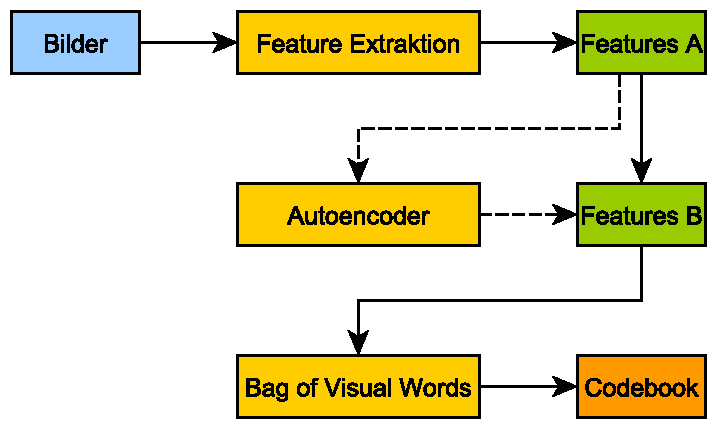
\includegraphics[scale=0.85]{images/model.pdf}
	\caption{Aufbau des Modells}
	\label{img:model}
\end{figure}

Das Erzeugen der \textit{Visual Words} aus einem Bild läuft in den ersten beiden Schritten analog ab, nur das die Menge \textit{Images} aus genau einem Bild, dem zu verarbeitenden, besteht. Die Features werden erst extrahiert und dann optional komprimiert. Für diese Schritte müssen auch exakt die gleichen Parameter verwendet werden, d.h.:

\begin{itemize}
	\item Der gleiche Feature-Detektor bzw. -Deskriptor muss gewählt werden.
	\item Eine Komprimierung muss stattfinden, wenn dies im Training der Fall. Andernfalls darf sie nicht erfolgen.
	\item Das gleiche Netzwerk zur Erzeugung der komprimierten Features muss gewählt werden.
\end{itemize}

In der dritten Phase verwendet der Bag of Visual Words das vorher generierte \textit{Codebook} und die Features aus der vorigen Phase um die \textit{Visual Words} zu ermitteln.

\section{Feature Extraktion}

Da es zahlreiche Verfahren zur Detektion und Extraktion von Features aus Bildern in Literatur und Praxis gibt, können diese unmöglich alle gleichermaßen Beachtung finden. In der Analyse wurde bereits auch aufgezeigt, dass über die Daten der HsH keine Annahmen getroffen werden können. Gegenstand dieser Arbeit soll daher die Objekterkennung im Bildern sein. Für diesen Zweck sollen im Weiteren zwei Deskriptoren ausgewählt werden:

\begin{itemize}
	\item Da die Schritte im Prozess aufeinander aufbauen, hängt die Qualität der Ergebnisse des Bag of Visual Word Verfahrens auch vom Autoencoder ab. Um den Bag of Visual Words an sich testen zu können, soll ein bereits kompakter, praktisch bewährter Deskriptor als Alternative dienen.
	\item Es ist denkbar, dass der Schritt der Komprimierung nicht in allen Fällen notwendig bzw. sinnvoll ist, da der Deskriptor bereits kompakt genug ist.
\end{itemize} 

Viele Verfahren erzeugen bereits einen kompakten Deskriptor. Beispielsweise ist die Komprimierung eines SIFT-Deskriptors (128 Komponenten) wahrscheinlich wenig erfolgreich: Der Autoencoder müsste 128 Neuronen im \textit{Input Layer} besitzen. Zur Komprimierung bleibt dann wenig \enquote{Platz} im Netz, es sei denn es werden mehrere \textit{Hidden Layer} verwendet, deren Neuronenanzahl zunächst ansteigt. Ziel soll es hier aber sein einen Deskriptor zu erzeugen, der zu Anfang viele Komponenten aufweist, um so einen Stacked Denoising Autoencoder zu trainieren, der mit jeder Schicht einen kompakteren Deskriptor liefert. Auf diese Weise können auch zum Experimentieren mehrere Deskriptoren generiert werden, deren Form von Anzahl der \textit{Hidden Layer} und deren Neuronenanzahl abhängt.\newline
Zhao \cite{aed2016} hat aus diesem Grund einen Feature-Vektor mit $3042$ erzeugt, der dann anschließend durch einen Autoencoder komprimiert wird. Die \textit{keypoints} werden hier durch den SIFT-Detektor ermittelt. Um jeden der \textit{keypoints} wird eine Nachbarschaft der Größe $41 \times 41$ betrachtet. Von diesen Ausschnitten werden die Gradienten in horizontale und vertikale Richtung bestimmt. Bei einem Einsatz eines Gaußfilters mit einer Filterkerngröße von $3 \times 3$, ergeben sich somit pro Richtung $1521$ Werte, die den Ausschnitt beschreiben. Der resultierende Feature-Vektor besitzt somit, für beide Richtungen, insgesamt $3042$ Komponenten.\newline
Um das Clustering-Verfahren auch ohne einen Autoencoder anwenden zu können, bzw. sicherzustellen, dass andere Feature-Deskriptoren für Bilder direkt verwendet werden können, soll in einem Test auch SIFT Gegenstand sein. So kann nicht nur die Qualität der Ergebnisse der beiden Deskriptoren verglichen werden, sondern auch Auswirkungen auf die Laufzeit des Bag of Visual Words.

\section{Autoencoder}

In diesem Ansatz wird ein Stacked Denoising Autoencoder zur Komprimierung eines Feature-Vektors entworfen, wie er in der Arbeit von Zhao \cite{aed2016} vorgeschlagen wurde. Hierfür wird zunächst im Abschnitt\enquote{Modell} ein objektorientiertes Modell entworfen, dass den Autoencoder, wie er in der Analyse beschrieben wurde, abbildet. Durch dieses Klassenstruktur lassen sich nun beliebige Autoencoder definieren, daher wird Im folgenden Teil \enquote{Parameter} auf den konkreten Autoencoder eingegangen, den Zhao entworfen hat.

\subsection{Modell}

\todo{Allgemein, train} Durch \textit{encode} wird der Autoencoder genutzt um die Testdaten zu komprimieren. Für praktische Anwendung ist es von Interesse, nur den Encoder-Teil anzuwenden, um auf Basis der komprimierten Darstellung eine Klassifikation oder Speicherung zu ermöglichen. \newline
Die Methode \textit{decode} kehrt den Prozess der Enkodierung wieder um. Auf diese Weise kann die erhaltene Rekonstruktion beispielsweise genutzt werden, um eine Beurteilung durch einen Menschen zu ermöglichen oder um mit dem Original verglichen zu werden.
  
\begin{figure}
	\centering
	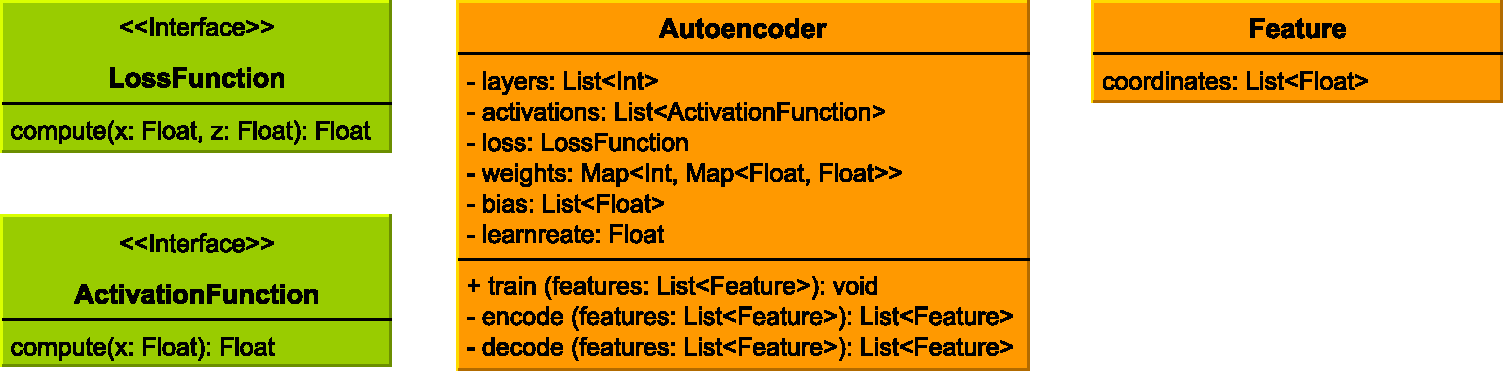
\includegraphics[scale=0.6]{images/ae_class.pdf}
	\caption{Klassendiagramm des Autoencoders}
	\label{img:ae_model}
\end{figure}

\subsection{Parameter}

\todo{Ein, zwei Intro Sätze} In einem Experiment wurde gezeigt, dass dieser Autoencoder \textit{state of the art} Ergebnisse erzielt: die Ergebnisse wurden unter verschiedenen Kriterien mit denen der Hauptkomponentenanalyse (PCA) und SIFT-PCA verglichen. Dabei erkannte der Autoencoder in fast allen die gleichen Features, jedoch durch einen 36 statt 128-elementigen Feature-Vektor. Aus diesem Grund soll Zhaos Autoencoder adaptiert werden.\newline
Der Encoder des vorgeschlagenen Modells besteht aus fünf Schichten, deren Neuronenanzahl sukzessive reduziert wird, bis schließlich die kleinste Schicht mit 36 Neuronen erreicht wird. Abbildung \ref{img:ae_model} zeigt die Schichten des Encoders sowie Decoders. Der Decoder ist umgekehrt aufgebaut und auch die Gewichte der Kanten zwischen zwei Neuronen entsprechen ihren Pendants im Encoder.

\begin{figure}
	\centering
	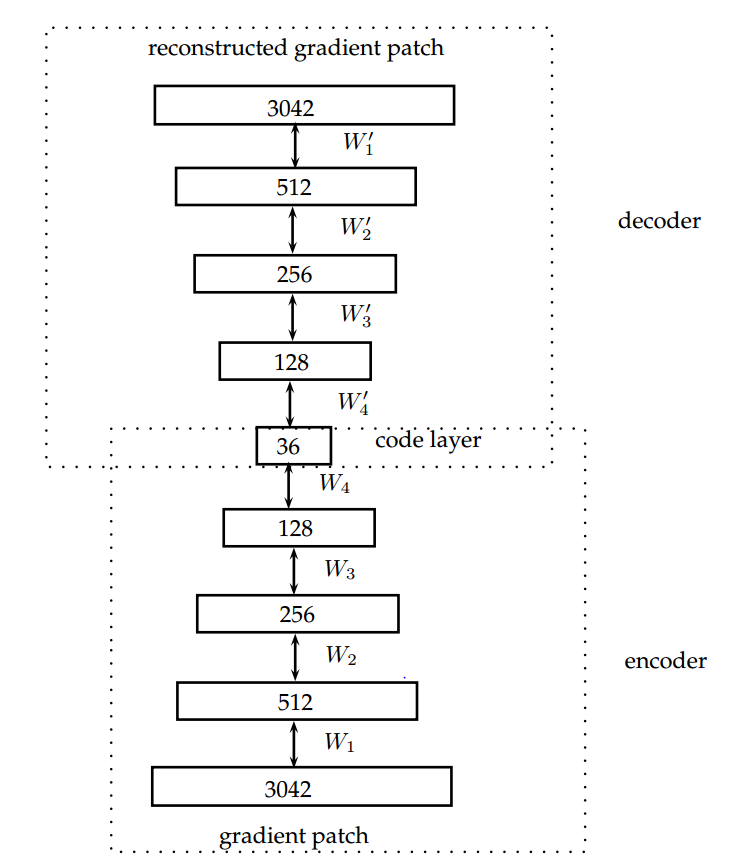
\includegraphics[scale=0.6]{images/ae_model.png}
	\caption{Schichten des verwendeten Autoencoders \cite{aed2016}}
	\label{img:ae_model}
\end{figure}

Die Hyperparameter für das verwendete Modell sind auch vollständig dokumentiert. Zhao verwendete hier für die Lernrate einen Wert von $2\%$, sodass $l = 0.02$. Für das Training der jeweiligen Autoencoderpaare werden verschieden viele Iterationen benutzt:
\begin{itemize}
	\item 1. Schicht: $1000$ Iterationen
	\item 2. Schicht: $700$ Iterationen
	\item 3. bis 5. Schicht: Je $500$ Iterationen
\end{itemize}
Als Größe für einen \textit{batch} wurde hier 128 gewählt, also sieht das Netz in einem \textit{foward} und \textit{backward pass} je 128 Trainingsexemplare. Da dies im Wesentlichen die Laufzeit durch eine Verwendung von mehr Speicher bewirkt, kann diese Zahl bei ungenügenden Ressourcen auch reduziert werden.

\subsection{TensorFlow}

TensorFlow ist ein Deep-Learning Framework, dass in Python geschrieben ist. Darüber hinaus gibt aus aber auch Schnittstellen zu anderen Sprachen wie beispielsweise C oder Java. Aus dem Namen leitet sich die bereits die Idee ab, die TensorFlow zugrunde liegt: Ein Tensor ist ein (multidimensionales) Array aus Daten. Diese Tensoren sind mit mathematischen Operationen, den Knoten, miteinander verbunden, sodass die Daten durch die Tensoren und Knoten \enquote{fließen} und dabei transformiert werden. Daher eignet sich TensorFlow hervorragend für die Darstellung neuronaler Netze: Die Kanten des Netzes entsprechen den Tensoren, die Neuronen in den Schichten führen mathematische Operationen auf den eingehenden Daten aus und leiten diese weiter an den nächsten Tensor. Die in TensorFlow definierten Modelle lassen sich sowohl auf mehreren CPUs sowie Nvidia GPUs ausführen. Hierfür ist es notwendig, dass auf dem System mindestens CUDA $7.5$ und die cuDNN Bibliothek $4.0$ installiert ist. 
TensorFlow folgt dem sogenannten \enquote{lazy} Programmierparadigma. Dies bedeutet, dass zunächst aus den Definitionen ein Modell aufgebaut wird. Dieses Modell kann durch TensorFlow automatisiert geprüft und visualisiert werden. Im nächsten Schritt werden alle nötigen Variablen initialisiert. Erst durch das Erzeugen und Aufrufen einer \enquote{Session} wird das Modell trainiert bzw. auf Testdaten ausgeführt.

\lstset{language=Python}
\begin{lstlisting}
import tensorflow as tf

a = tf.placeholder(tf.int16)
b = tf.placeholder(tf.int16)

addOp = tf.add(a, b)

init = tf.initialize_all_variables()

with tf.Session() as sess:
    sess.run(init)
    print "Addition: %i" % sess.run(addOp, feed_dict={a: 2, b: 3})

sess.close()
\end{lstlisting}

\section{Bag of Visual Words}

In der Analyse wurde bereits sequentielle Varianten des Lloyd und Histogramm Algorithmus vorgestellt und aufgezeigt, an welchen Stellen eine Parallelisierung der Berechnung durch Grafikkarten erfolgen kann. Im Folgenden wird aus diesen Informationen je Algorithmus eine parallele Version abgeleitet, welche sich für die Realisierung als CUDA Programm eignen.
Im Abschnitt Modell wird dann der Aufbau des Modells und Ablauf der Funktionsaufrufe skizziert. Zur Interaktion stehen einem Anwender im Wesentlichen eine Funktion zu Generierung eines Modells und zur Berechnung der \textit{Visual Words} eines Bildes zur Verfügung.

\subsection{Parellisierung von Llyods Algorithmus}

Der Thread in einem Block mit der \textit{threadId} 0 fungiert hier als Master für die anderen Threads. Die Initialisierung der Cluster mit zufälligen Vektoren aus $v$ wird ebenfalls von diesem übernommen. Die Zuweisung von Vektoren zu Clustern nimmt $\Theta(nk)$ Zeit in Anspruch, wobei $n$ die Anzahl Vektoren und $k$ die Anzahl der Cluster ist. Diese Phase kann parallelisiert werden, in dem pro Feature Vektor ein Thread verwendet wird: Jeder Thread berechnet für seinen Feature Vektor die Distanz zu allen Clusterschwerpunkten und bestimmt den Index des Clusters, der am Nächsten ist. Dieser Prozess ist in Pseudocode in Zeile 6 bis 8 ausgedrückt. Bevor die Cluster aktualisiert werden, müssen die Threads synchronisiert werden: Andernfalls ist nicht garantiert, dass die Berechnung jedes Threads abgeschlossen ist.

\lstset{language=C}
\begin{lstlisting}[mathescape=true]
kmeans_gpu
	if threadId == 0
		$c_{j} = rand(p_{i}) \in P, \: j = 1,...,k, \: c_{j} \neq c_{i} \: \forall i \neq j$
	synchronize threads
	until convergence
		for each $x_{i} \in P_{threadId}$
			$l_{i} = argminD(c_{j}, p_{i})$
		synchronize threads
		if threadId == 0
			for each $p_{i} \in P$
				$c_{l_{i}} = c_{l_{i}} + p_{i}$
				$m_{l_{i}} = m_{l_{i}} + 1$
			for each $c_{j} \in C$
				$c_{j} = \frac{1}{m_{j}} c_{i}$
\end{lstlisting}

\subsection{Parallele Reduzierung von Histogrammen}

Die Berechnung eines Histogramms kann parallelisiert werden, da die Operation assoziativ und kommutativ ist: Es spielt keine Rolle in welcher Reihenfolge die Daten abgearbeitet werden bzw. in welcher Reihenfolge die Klassen inkrementiert werden. Wenn das zu beschreibende Histogramm im \textit{global memory} vorliegt, wird die Berechnungsgeschwindigkeit stark reduziert, da viele Threads auf die gleichen Speicheradressen des Histogramms schreibend zugreifen. Damit es nicht zu Lese- / Schreibanomalien kommt, muss das Inkrementieren einer Klasse atomar sein, d.h. zwischen Lese- und Schreibzugriff darf kein anderer Thread auf die Adresse zugreifen. Dies wird in CUDA durch die Operation \textit{atomicAdd} realisiert. Damit die Anzahl an Threads die auf dieselbe Adresse schreiben eingeschränkt wird, arbeitet jeder Block auf einem lokalen Histogramm im \textit{shared memory}. Wenn alle Blöcke ihre lokalen Histogramme berechnet haben, müssen diese noch in das Histogramm im \textit{global memory} kumuliert werden. \todo{Listing kurz erklären.}

\lstset{language=C}
\begin{lstlisting}
__global__
void histogram_kernel (float *features, float *clusters, unsigned int *histo, int featureSize, int count, int k) {
	extern __shared__ int *sharedMemory[];
	unsigned int histo_private = (unsigned int*) sharedMemory;
	
	if (threadIdx.x < k) {
		histo_private[threadIdx.x] = 0;		
	}
	__syncthreads();

	int id = threadIdx.x + blockDim.x * gridDim.x;
	int stride = blockDim.x * gridDim.x;
	
	while (i < count) {
		float *feature = &features[i * featureSize];
		int bin = findNearestCluster(feature, clusters, featureSize, k)); 
		atomicAdd(&(histo_private[bin]), 1);
		i += stride;	
	}
	__syncthreads();
	
	if (threadIdx.x < k) {
		atomicAdd(&(histo[threadIdx.x]), histo_private[threadIdx.x]);		
	}
}
\end{lstlisting} 

\subsection{Aufbau des Bag of Visual Words Algorithmus}

Der Aufbau des Bag of Visual Words Modell ist als Klassendiagramm in Abbildung \ref{img:bovw_class} dargestellt. Cluster und Features werden hier als Punkte in einem $n$-dimensionalen Raum aufgefasst, deren Position durch eine Liste von $n$ \textit{float}-Werten definiert ist. Diese Gemeinsamkeit wird durch Point abstrahiert. Ein Objekt der Klasse Cluster enthält zusätzlich eine Liste \textit{members}, welche die Features enthält, die dem Cluster zugeordnet sind.
Die BagOfVisualWords-Klasse selbst umfasst nur \textit{host code} und steuert den Prozessablauf. Die Kmeans-, Histogramm- und Shared-Klasse enthalten die CUDA \textit{kernels} und führen die Berechnungen auf der GPU aus.\newline
Die folgenden Abschnitte \enquote{Generierung des Modells}, \enquote{Speichern und Laden eines Modells} und \enquote{Berechnung der Visual Words} illustrieren die Kernfunktionalitäten der BagOfVisualWords-Klasse sowie den jeweiligen Prozessablauf anhand des Klassendiagramms.

\begin{figure}
	\centering
	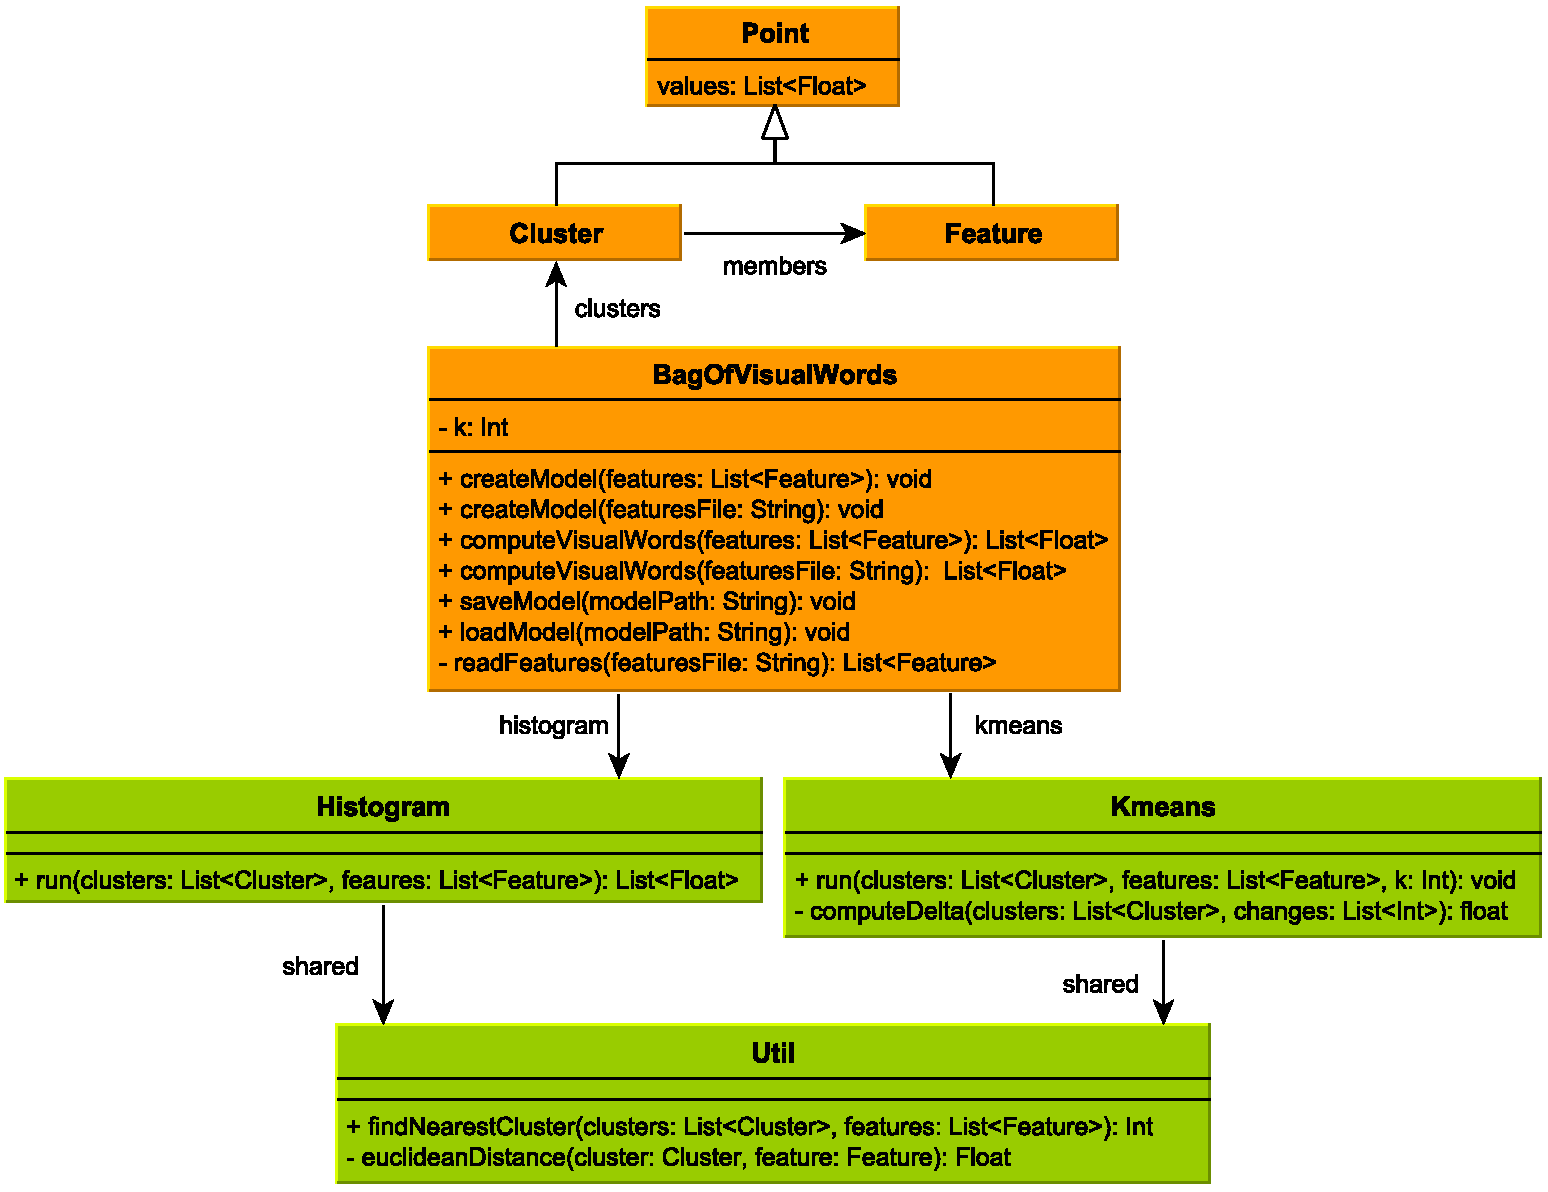
\includegraphics[scale=0.57]{images/bovw_class.pdf}
	\caption{Klassendiagramm des Bag of Visual Words}
	\label{img:bovw_class}
\end{figure}
 
\subsubsection{Generierung des Modells}

Die Generierung eines Modells kann durch die Funktion \textit{createModel} gestartet werden. Die Funktion ist überladen und erwartet als Parameter entweder eine Liste der Features oder den Pfad zu einer Datei, in der die Features gespeichert sind. Der Ablauf der Methodenaufrufe ist dann wie folgt:

\begin{itemize}
	\item Es werden bei Aufruf mit einem String die Features eingelesen und anschließend \textit{generateModel} mit dieser Feature-Liste aufgerufen. Der kmeans Algorithmus wird mit den Features und \textit{k} aufgerufen. Die Daten werden zum \textit{device} kopiert und der Prozess gestartet. 
	\item Kmeans nutzt die ausgelagerte Funktion \textit{findNearestCluster} um den nächsten Cluster eines jeden Features zu bestimmen. Intern wird hier durch \textit{computeEuclideanDistance} die Entfernung eines Cluster-Feature-Paares bestimmt.
	\item Anschließend prüft \textit{computeDelta} ob sich die Zuordnung von Features zu Clustern nicht mehr wesentlich geändert hat, d.h. die relative Veränderung unter dem Schwellwert liegt.
	\item Ist der Schwellwert oder eine maximale Anzahl an Iterationen erreicht, ist der Prozess abgeschlossen und die \textit{device} Cluster werden in die Cluster des aufrufenden BagOfVisualWords-Objektes kopiert.
\end{itemize}
 
\subsubsection{Speichern und Laden eines Modells}

Um Modelle über den Speicher hinaus verwenden zu können, soll die Funktion angeboten werden, diese persistent zu speichern und wieder einlesen zu können. Die Methode \textit{saveModel(modelPath: String)} der BagOfVisualWords-Klasse speichert die Anzahl der Cluster \textit{k}, die Liste der Cluster \textit{clusters} sowie die Zuordnung der Features \textit{members} unter dem Pfad \textit{modelPath}. Durch das Pendant \textit{readModel(modelPath: String)} kann ein so gespeichertes Modell, also \textit{k}, \textit{clusters} und \textit{members}, wieder eingelesen werden.\newline
So ergibt sich zum Beispiel für ein $k = 5$ und 100 Features mit je 128 Komponenten, eine Datei mit 106 Zeilen: Die erste Zeile enthält \textit{k}. Darauf folgen \textit{k} viele, also hier fünf, Zeilen mit den Zentren der Cluster und anschließend 100 Zeilen mit den Features. Die Zeilen mit den Clustern enthalten hier 128 Werte, durch Leerzeichen separiert. Die Features enthalten einen Wert am Ende der Zeile mehr: Diese Ganzzahl gibt den Index des Clusters an, zu der das Feature gehört.

\subsubsection{Berechnung der Visual Words}

Die Erzeugung der \textit{Visual Words} wird durch die BagOfVisualWords-Klasse angestoßen. Wie bei der Modellgenerierung wird intern ein CUDA-Programm, die Histogram-Klasse, verwendet. Für den Gebrauch muss die \textit{computeVisualWords} Methode aufgerufen werden. Der Ablauf ist dann wie folgt:

\begin{itemize}
	\item Wie beim kmeans Algorithmus kann \textit{computeVisualWords} der BagOfVisualWords-Klasse mit einer Liste der Features oder dem Pfad zu einer Feature-Datei aufgerufen werden. Letztere ließt die Features ein und ruft dann wiederum \textit{computeVisualWords} mit der Feature-Liste auf. Es wird geprüft, ob ein Modell vorhanden ist, also eine Liste von Clustern vorliegt. Ist dies nicht der Fall, wird abgebrochen.
	\item Die \textit{run} Methode der Histogram-Klasse wird nun mit den \textit{clustern} der aufrufenden BagOfVisualWords-Instanz und den Features aus dem vorigen Schritt aufgerufen. Um das \textit{Visual Word} für ein Feature zu bestimmen, wird \textit{findNearestCluster} aus der Shared-Klasse genutzt. Da diese Funktion den Index des Clusters zurückgibt, kann dieser direkt für die zu inkrementierende Position im Histogramm verwendet werden.
	\item Das Histogramm wird zum \textit{host kopiert} und an den Aufrufer zurückgegeben. Es kann nun gespeichert oder für weitere Analyse verwendet werden.
\end{itemize}
\chapter{Implementierung}

Die Implementierung behandelt in zwei Teilen die Umsetzung des Bag of Visual Word Modells in CUDA und des Autoencoders in TensorFlow. In beiden Abschnitten wird zunächst wird die Extraktion der Features anhand von Quellcode beschrieben. Im Bag of Visual Word Teil folgt eine Betrachtung der \textit{kernels} des k-means Algorithmus sowie Unterschiede in der Implementierung zwischen \textit{global} und \textit{shared memory}. Im Teil zum Autoencoder folgt nach der Beschreibung der Feature-Aufbereitung das Modell in TensorFlow.

\todo{Why CUDA C, TensorFlow Python}
\todo{CUDA C ist eine sehr hardwarenahe Sprachen, Python ist eine interpretierte Hochsprache und TensorFlow generiert den entsprechenden Code für die Grafikkarte.}

\section{Extraktion der Patches}

Zu Ermittlung der \textit{keypoints} durch den SIFT-Detektor wird auf die \textit{opencv}\footnote{https://github.com/TODO/opencv} Implementierung von SIFT zurückgegriffen. Zur Verwendung des SIFT Algorithmus ist es erforderlich das \textit{opencv} Projekt zusammen mit dem \textit{opencv-contrib}\footnote{https://github.com/TODO/opencv-contrib} Projekt selbst zu kompilieren. Bei SIFT handelt es sich um einen patentierten Algorithmus, daher ist er seit Version 3.0 nicht mehr standardmäßig im \textit{opencv} Projekt enthalten.

Da der Autoencoder in Python geschrieben ist, erfolgt die Gewinnung der Patches in der gleichen Sprache, um so eine einfache weitere Verarbeitung zu ermöglichen. Der Prozess lässt sich in drei Schritte untergliedern. Um alle Features eines Bildes zu erhalten, wird die Funktion \textit{extractFeatures} mit dem Pfad zu einer Bilddatei ausgerufen. Es wird das Bild eingelesen, konvertiert und durch den \textit{opencv} SIFT-Detektor die \textit{keypoints} ermittelt. Die Berechnung der Gradienten der Nachbarschaften um diese \textit{keypoints} erfolgt dann durch die Funktion \textit{computeDescriptors}:

\lstset{language=Python}
\begin{lstlisting}
def computeDescriptors(image, keypoints):
  descriptors = []
  
  for keypoint in keypoints:
  	patch = getPatch(image, keypoint)
  	gradients = computeGradients(patch)
  	descriptors.append(gradients)
  return descriptors
  
def getPatch (image, keypoint):
  x, y = keypoint.pt[0], keypoint.pt[1]
  return image[y-20:y+21, x-20:x+21]
\end{lstlisting}

Für jeden \textit{keypoint} werden nun wiederum \textit{Patches} berechnet: Hierbei handelt es sich um die Nachbarschaften der Größe $41 \times 41$. Die Gradienten in vertikale und horizontale Richtung eines solchen \textit{Patches} werden durch \textit{computeGradients} bestimmt. In Zeile 2 und 3 in Abbildung \ref{lst:compGrad} findet die Konvolution des Patches mit dem Sobel-Operator statt, den \textit{opencv} anbietet.

\lstset{language=Python,label={lst:compGrad}}
\begin{lstlisting}
def computeGradients(image):
  grad_x = cv2.Sobel(image, cv2.CV16S, 1, 0)
  grad_y = cv2.Sobel(image, cv2.CV16S, 0, 1)
  return [grad_x, grad_y]
\end{lstlisting}

In Abbildung \ref{img:gradients} sind auf der rechten Seite sind, in zwei Reihen, einige der gefundenen Gradienten des Bildes auf der linken Seite dargestellt. Dadurch, dass das Bild des Stop-Schildes viele deutliche Kanten aufweist, sind die Gradienten leicht zuzuordnen.

\begin{figure}
	\centering
	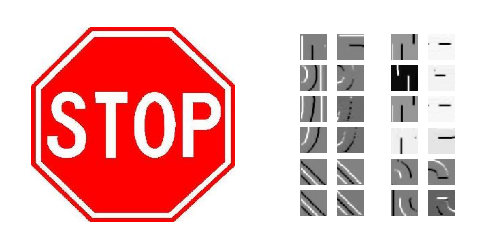
\includegraphics[scale=0.65]{images/gradients_patch.png}
	\caption{Stop-Schild und Gradienten um einige der gefundenen \textit{keypoints}.}
	\label{img:gradients}
\end{figure}

Sollte im späteren eine Umsetzung des Autoencoders in CUDA C erfolgen, so lässt sich die Gewinnung der Patches leicht portieren. Die Verwendung von SIFT erfolgt in C analog (in entsprechender Syntax).

\section{Autoencoder}

In diesem Kapitel wird behandelt wie der Autoencoder in Python und TensorFlow umgesetzt wurde. Zunächst wird auf die Erhebung der Feature-Vektoren unter Verwendung der \textit{opencv}-Bibliothek eingegangen. Anschließend erfolgt eine Übersicht des Python-Codes zur Definition des Autoencoders.

\subsection{Projektstruktur} Das Python-Projekt für des Autoencoders besteht aus fünf Dateien. In autoencoder.py ist eine gleichnamige Klasse zur objektorientierten Verwendung enthalten. Die Funktionen zur Feature-Extraktion sind in der Datei feature\textunderscore extractor.py und werden im folgenden Abschnitt näher behandelt. Die Datei util.py stellt eine Sammlung allgemein verwendeter Funktionen bereit, z.B. zur Messung von Zeit oder Konvertierung von Datenstrukturen. Wie beim Bag of Visual Words liegt hier eine main-Datei bei, welche die Benutzung des Autoencoders durch die Kommandozeile erlaubt.

\dirtree{%src
.1 src.
.2 autoencoder.py.
.2 test.cpp.
.2 main.py.
.2 util.py.
}

Öffentlich kann auf einem erstellten Autoencoder aus der autoencoder.py Datei die Funktion \textit{fit(train\textunderscore data)} sowie \textit{transform(test\textunderscore data)} aufgerufen werden. Erstere verwendet dabei das Argument \textit{train\textunderscore data} um die Gewichte anhand der Daten zu initialisieren.  Durch \textit{transform} wird dann der Enkodierungsprozess auf \textit{test\textunderscore data} angewendet und liefert pro Feature einen 36-elementigen Feature-Vektor. Entsprechend des Entwurfs muss es sich bei \textit{train\textunderscore data} und \textit{test\textunderscore data} um eine Liste von Feature-Vektoren mit je 3042 Elementen pro Vektor handeln.

\subsection{Modell in TensorFlow}

Zur Implementierung des Autoencoders wurde TensorFlow verwendet. TensorFlow ist ein DeepLearning Framework und bietet Schnittstellen in diversen Sprachen an. Neben OpenCL wird auch NVIDIAs CUDA unterstützt, sodass TensorFlow Programme automatisch von Grafikkarten profitieren können, ohne das der Entwickler diese explizit berücksichtigen muss. Für diese Umsetzung eines Autoencoders wurde Python und das Projekt \textit{libsdae-autoencoder-tensorflow}\footnote{https://github.com/rajarsheem/libsdae-autoencoder-tensorflow} von Rajarshee Mitra genutzt. Unter Berücksichtigung der bekannten Parameter aus dem Konzept, ergibt sich die folgende Definition eines Modells:

\lstset{language=Python}
\begin{lstlisting}
from deepautoencoder import StackedAutoEncoder
import cv2
import numpy
import featureExtractor

imagePaths = []

features = featureExtractor.extractAll(imagePaths)
index = numpy.random.rand(features.shape[0]) < 0.8
train = features[index]
test = features[~index]

model = StackedAutoEncoder(
  dims=[3042, 1024, 512, 128, 36],
  activations=['relu', 'relu', 'relu', 'relu', 'relu'], 
  epoch=[1000, 1000, 700, 700, 500], 
  loss='rmse', 
  lr=0.02, 
  batch_size=100
)

model.fit(train)
result = model.transform(test)
\end{lstlisting}

In Zeile 8 wird die bereits eingeführte Funktion \textit{extractAll} genutzt, um alle Features der Bilder, die in \textit{imagePaths} enthalten sind, zu gewinnen. Diese werden in der Zeile 10 bzw. 11 in eine Test- und Trainingsmenge aufgeteilt, wobei erstere 80\% und letztere 20\% der Bilder enthält.
In den Zeilen 12 bis 19 findet die Definition des Autoencoders statt. Der \textit{StackedAutoEncoder} entstammt hierbei dem Eingangs erwähnten Projekt von Rajarshee Mitra. In \textit{dims} wird die Menge der Schichten des Encoder-Teils durch eine Liste von Ganzzahlen dargestellt: Eine Zahl steht für die Anzahl der Neuronen pro Schicht. Hier wird davon ausgegangen, dass benachbarte Schichten voll verbunden sind. Der Decoder-Teil ist umgekehrt aufgebaut, daher leitet sich dieser aus der Encoder-Definition ab und muss nicht notiert werden. Folglich werden in \textit{activations} die Aktivierungsfunktion auch nur einmal notiert. 

Die Abkürzung \textit{relu} steht hier für Rectified Linear Unit (ReLU). ReLU wird in vielen Netzen, wie auch hier, verwendet. Negative Werte sowie Gradienten die gegen unendlich gehen, wie beispielsweise bei der Sigmoidfunktion möglich, werden vermieden. 

Da über die Anzahl der Iterationen die pro Autoencoder-Paar im Training ausgeführt werden soll, keine Angaben vorliegen, wurden hier Zahlen getestet die üblich sind. 

Durch eine Variation der Iteration in mehreren Testläufen kann eine Zahl ermittelt werden, die ein gutes Verhältnis von Fehlerrate zu Ausführungszeit bietet: Gerade in den Ersten schichten des Encoders, bzw. den Letzten des Decoders, sind erheblich mehr Verbindungen vorhanden. 

In Zeile 17 wird unter \textit{loss} die die Metrik definiert, mit welcher der Fehler der Rekonstruktion gemessen wird. \textit{rmse} steht für \textit{root-mean-square error} und ist somit der gemittelte quadratische Fehler. 

Die Lernrate wird hier mit \textit{lr} bezeichnet und wurde entsprechend des konzipierten Autoencoders auf 2\% gesetzt.

In Zeile 22 wird \textit{fit} aufgerufen um das Modell mit den \textit{train} Features zu trainieren. Hierbei kann optional durch \textit{print\textunderscore step} angegeben werden, nach wie vielen Iterationen im Training pro Autoencoder-Paar die Fehlerrate ausgegeben werden soll.
Anschließend wird der Autoencoder genutzt um die Testdaten einmal zu komprimieren und wieder zu rekonstruieren. Auf diese Weise kann \textit{result} zum Beispiel genutzt werden, um eine Beurteilung durch einen Menschen zu ermöglichen: Handelt es sich wie hier um Bilder von Gradienten, können so Original und Rekonstruktion nebeneinander gestellt als Bild gespeichert werden. Für praktische Anwendung ist es interessanter, nur den Encoder-Teil anzuwenden, um auf Basis der komprimierten Darstellung eine Klassifikation oder Speicherung zu ermöglichen.  

\section{Bag of Visual Words}

Zunächst wird eine Übersicht über die Projektstruktur und die BagOfVisualWords-Klasse gegeben. Damit ein Modell über den Speicher hinaus verwendbar ist, wird ein einfacher Mechanismus zur Persistierung vorgestellt. Anschließend werden die Wesentlichen Bag of Visual Words Funktionen betrachtet. Da die Feature-Extraktion Voraussetzung für beide Anwendungsfälle ist, wird im folgenden Abschnitt eine Implementierung auf Basis der \textit{opencv}-Bibliothek angeführt. Darauf Aufbauend folgt eine Übersicht des k-means Clustering der Features. Unterschiede sowie Limitierungen der \textit{global} und \textit{shared memory} Implementierungen werden hier anhand des Codes aufgezeigt.

\subsection{Projektstruktur}

Der Bag of Visual Words ist als Klasse in C++ umgesetzt worden und ist auch die öffentliche API des Programms. Der k-means und Histogramm Algorithmus sind CUDA C Programme und tragen somit die Endung .cu. Neben den CUDA Programmen sind hier aber auch Varianten in C zur Ausführung auf CPUs enthalten. In der util.cpp Datei sind Funktionen zur Messung von Ausführungszeiten, Lesen / Schreiben von Dateien und und Formatierung von Zeichenketten enthalten. Zur direkten Ausführung im Projekt ist eine main.cpp Datei enthalten. Hier werden Argumente der Kommandozeile geparst, um einen entsprechenden Bag of Visual Words zu generieren bzw. auszuführen. Inklusive header-Dateien ergibt sich somit folgender Aufbau des src-Ordners:
\dirtree{%src
.1 src.
.2 BagOfVisualWords.h.
.2 BagOfVisualWords.cpp.
.2 histogram.h.
.2 histogram.cu.
.2 kmeans.h.
.2 kmeans.cpp.
.2 main.cpp.
.2 util.cpp.
}

\subsection{Verwendung und wesentliche Klassen}

Zur Verwendung wird ein Objekt der BagOfVisualWords-Klasse durch Aufruf des Konstruktors angelegt. Hierbei muss die Anzahl der Cluster $k$ übergeben werden. Standardmäßig werden bei Erstellung und Nutzung eines Modells die CUDA Versionen des k-means und Histogramm Algorithmus aufgerufen. Zu Vergleichszwecken können aber auch die CPU-basierten Varianten durch \textit{setMode(1)} ($0 = GPU, 1 = CPU$) verwendet werden. Die Erstellung eines Modells kann dann durch Aufruf von \textit{createModel(Mat features)} oder \textit{createModel(string featurePath)} erfolgen. Letztere liest aus der Datei \textit{featurePath} zeilenweise die Pfade von Bilddateien ein und extrahiert die Features dieser durch die private Funktion \textit{extractFeatures}. Aus diesen wird die Matrix \textit{features} für das folgende Clustering erzeugt.
Zur Erzeugung des \todo{Visual Words Histogramms} dient die Methode \textit{computeViusalWords(string imagePath)}. Auch hier werden wieder durch \textit{extractFeatures} die Features aus dem Bild \textit{imagePath} extahiert und anschließend, je nach Modus durch GPU oder CPU, dass Histogramm berechnet. 

\todo{move Kozept?} Damit ein Modell nicht immer erneut aufgebaut werden muss, wenn es öfter verwendet wird, kann es als Textdatei gespeichert werden. Dafür kann auf einem Objekt der BagOfVisualWords-Klasse \textit{writeModel(string modelPath)} aufgerufen werden. Die Schwerpunkte der Cluster werden zeilenweise in die Datei \textit{modelPath}/clusters geschrieben, sodass sich $k$ Zeilen mit 128 Elementen bei der Verwendung von SIFT ergeben. Die Mitgliedschaften der Features zu Cluster wird in der Datei \textit{modelPath}/membership gespeichert und enthält so viele Zeilen wie Features vorliegen. Jede Zeile enthält die $x$ und $y$ Koordinaten des \textit{keypoints} und den Index des zugehörigen Clusters. Der Index bezieht sich hierbei auf die Position des Clusters in der Datei \textit{modelPath}/clusters.

\subsection{Paralleler k-means Algorithmus}

Als Referenzimplementierung für die Umsetzung in CUDA C diente hier das Projekt von \todo{[REF]}. Durch \todo{Methodenname} wird ein k-means Clustering auf der GPU ausgeführt. Der Algorithmus erwartet dabei als Parameter:

\begin{itemize}
	\item \textbf{float *features} Eine Liste von Feature-Vektoren, die zu gruppieren sind.	
	\item \textbf{float *clusters} Eine Liste, welche mit den Clustern befüllt wird.
	\item \textbf{int featureSize} Die Anzahl der Komponenten in einem Feature-Vektor.
	\item \textbf{int k} Die Anzahl der zu bildenden Cluster $k$.
	\item \textbf{int iterations} Die maximale Anzahl an Iterationen, die durchlaufen wird, falls bisher keine Konvergenz erreicht wurde.
	\item \textbf{float conv} Ein Schwellwert, der in jeder Iteration mit der relativen Veränderung der Mitgliedschaft verglichen wird. Ist er größer, wird das Clustering beendet.
\end{itemize}

Vor dem Aufruf des \textit{kernels} wird für die Features und Cluster der notwendige Speicher allokiert und die Daten zum \textit{device} kopiert. Die Dimensionen der Features sowie der Cluster werden durch \textit{Float}-Werte dargestellt. Ein SIFT Feature-Vektor belegt so $128 \times 4 = 512$ Byte. Der Deskriptor, der durch den Autoencoder erzeugt wurde belegt $36 \times 4 = 144$ Byte. Da die Features ursprünglich als zweidimensionales Array vorliegen (\textit{Float-Pointer-Pointer}), müssen diese in ein eindimensionales Arrays konvertiert werden, damit die Daten korrekt von \textit{host} zu \textit{device} kopiert werden können. 
\todo{Übergang} Von diesen sind drei CUDA kernels, also Funktionen die durch die Grafikkarte ausgeführt werden. Diese Funktionen werden solange in einer Schleife durchlaufen, bis das Konvergenzkriterium erfüllt wurde.

\begin{itemize}
	\item \textbf{Distanzberechnung} euclideanDistance(float *points, float *clusters) Die Distanz wird zwischen jedem Punkt und Cluster ermittelt. Es wird für jeden Punkt der Index des Clusters zurückgegeben, der am Nächsten ist.
	\item \textbf{Cluster-Mitgliedschaft} findNearestCluster() agiert auf jeweils einem Feature. Der Index des Features ist somit von der $threadIdx$ abhängig und berechnet sich unter Berücksichtigung der Blockdimension als $blockDim.x * blockIdx.x + threaIdx.x$. Es wird der nächste Cluster zum Feature berechnet und auch bestimmt, ob sich die Zuordnung des Features verändert hat.
	\item \textbf{Konvergenzkriterium} computeDelta() ermittelt die relative Veränderungen der Feature-Cluster Mitgliedschaft. Ist dieser Wert kleiner als ein vorgegebener \todo{PARAM, Schwellwert} oder wurde die maximale Anzahl an Iterationen \textit{iterations} erreicht, ist das Clustering abgeschlossen, andernfalls wird fortgefahren.
\end{itemize}

Die Anzahl der veränderten Mitgliedschaften wird anschließend zurück zum \textit{host} kopiert. Diese Zahl wird durch die Gesamtanzahl der Features dividiert, um so die relative Veränderung zu bestimmen. 

\subsection{Shared memory}

Zur Beschleunigung der Berechnung bei der Suche des nächsten Clusters zu einem gegebenen Punkt, soll CUDAs \textit{shared memory} genutzt werden. Hierfür werden die Cluster pro Block vom \textit{global} in den \textit{shared memory} kopiert. Daraus ergibt sich eine Anpassung an mehreren Stellen im Programm. \todo{Globaler C Switch.} Die Größe des extra zu allokierenden Speichers pro Block muss in \textit{blockSharedDataSize} berücksichtigt werden und ergibt sich aus der Anzahl der Cluster und der Anzahl der Elemente eines Features:

\lstset{language=C}
\begin{lstlisting}
const unsigned int membershipDataSize = numThreads * sizeof(unsigned char);
const unsigned int clusterDataSize = k * size * sizeof(float);
const unsigned int blockSharedDataSize = membershipDataSize + clusterDataSize;
\end{lstlisting}

In der Funktion \textit{findNearestCluster} wird der Parameter \textit{clusters} in \textit{deviceClusters} umbenannt. Vor der Berechnung der Mitgliedschaft wird nun ein lokaler Pointer \textit{clusters} angelegt und alle notwendigen Cluster kopiert.

\lstset{language=C}
\begin{lstlisting}
float *clusters = (float *)(sharedMemory + blockDim.x);
for (int i = threadIdx.x; i < k; i += blockDim.x) {
  for (int j = 0; j < size; j++) {
    clusters[k * j + i] = deviceClusters[k * j + i];
  }
}
__syncthreads();
\end{lstlisting}

Da die Größe von \textit{clusterDataSize} hier von $k$ und $size$ abhängt, also der Anzahl der Cluster und der Anzahl der Komponenten eines Features, ist diese Implementierung nur einsetzbar, wenn $k$ und $size$ in Hinsicht auf den verfügbaren \textit{shared memory} nicht zu groß gewählt werden. Die Größe von \textit{membershipDataSize} ist nur abhängig von der Anzahl der Threads. Werden beispielsweise 256 Threads pro Block gewählt, benötigt dies konstant, unabhängig von $k$ und $size$, 1024 Byte \textit{shared memory}. Für die hier verwendeten Deskriptoren kann somit eine Obergrenze für $k$ berechnet. Gängige Modelle CUDA kompatibler Grafikkarten sind mit 16 oder 48 Kilobyte \textit{shared memory} ausgestattet. Von 256 Threads pro Block ausgehend ergibt dies ein maximales $k$ von $(memory - 1024) / 512$. Für SIFT sind dies bei 48 Kilobyte maximal 91, für 16 Kilobyte 29 Cluster. Der von Zhao entworfene Deskriptor ermöglicht bei 48 Kilobyte Speicher bis zu 326 Clustern, für 16 Kilobyte bis zu 104. Sind dennoch mehr Cluster notwendig, muss auf die \textit{global memory} Implementierung zurückgegriffen werden. Hier werden, je nach Anzahl der Cluster, erheblich höhere Berechnungszeiten erwartet, jedoch gibt es kein Limit für die Gesamtanzahl an Clustern.
\chapter{Evaluierung}

Die Qualität der Ergebnisse des in der Implementierung realisierten Modells wird in diesem Kapitel durch ein Testexperiment überprüft. Weiterhin werden Ausführungszeiten für beispielsweise verschieden große $k$ beim Bag of Visual Words betrachtet, um eine Einsicht in die Performance der Algorithmen zu gewinnen.
Im Kapitel Experimentaufbau wird zunächst das Experiement sowie verwendete Metriken und Ergebnistypen behandelt. Nachfolgend wird erläutert, wie die großen Menge an benötigten Trainings- und Testdaten wiederholbar und automatisiert aufgebaut wird. Dieser Abschnitt illustriert auch, wie eine Durchführung des Experiments vonstatten geht. Im letzten Teil werden dann konkrete Testgruppen aus den Caltech101 \cite{cal2004} Bilddaten erzeugt. Diese Menge an Bilddaten hat große Verbreitung im Bereich der Objekterkennung gefunden. Auf diese Weise ist ein Vergleich mit Arbeiten Anderer prinzipiell möglich.

\section{Testdaten und Testgenerierung}

Der Abschnitt Testdaten stellt die hier verwendete Menge von Bildern vor, die Caltech101, welche extra für den Test von Algorithmen bezüglich der Objekterkennung in Bildern entwickelt wurde.\newline
Im folgenden Abschnitt zur Testgenerierung wird ein Verfahren zur zufälligen Auswahl von Trainings- und Testbildern unter Berücksichtigung verschiedener Restriktionen, wie z.B. dem Verhältnis der Anzahl von Trainings- zu Testbildern vorgestellt.

\subsection{Testdaten}

Als Testmenge wurden die Bilder der Caltech101-Menge verwendet. Bei Caltech101 handelt es sich um eine weit verbreitete Menge von Bilddaten, die vorwiegend zum Test von Algorithmen bezüglich der Objekterkennung in Bildern dient. Insgesamt liegen, wie der Name sagt, 101 Kategorien vor, die jeweils zwischen 40 und 800 Bildern enthalten. Auf der offiziellen Webseite \footnote{http://www.vision.caltech.edu/Image\textunderscore Datasets/Caltech101/} und im Artikel der Autoren wird empfohlen, die eigene Arbeit mit derer anderen vergleichbar zu halten, indem:

\begin{itemize}
	\item Eine feste Anzahl an Trainings- und Testbildern verwendet wird.
	\item Experimente mit einer zufälligen Auswahl an Bildern wiederholt werden.
	\item Ähnlich viele Bilder, wie in den Arbeiten anderer, verwendet werden (1, 3, 5, 10, 15, 20 oder 30 Trainingsbilder; 20 oder 30 Testbilder).
\end{itemize}

Die Caltech101 Daten liegen nach Download kategorisiert im JPG-Format vor. Die Struktur wurde so beibehalten und ist noch für die Testgenerierung relevant. Direkt unter dem Caltech101-Ordner ist pro Kategorie ein Ordner vorhanden, der die jeweiligen Bilder immer im gleichen Namensschema enthält:\newline

\dirtree{%src
.1 Caltech101.
.2 accordion.
.3 image\textunderscore 0001.jpg.
.3 image\textunderscore 0002.jpg.
.3 ....
.2 airplanes.
.3 ....
.2 ....
}

Abbildung \ref{img:strawberries} zeigt vier Bilder aus der Kategorie \enquote{Erdbeere}. Neben Bildern von realen Rosengewächsen sind auch Zeichnungen und Objekte enthalten, die Form und Farbe der Erdbeere nachempfunden sind. Auch sind die Objekte auf einem Bild zum Teil in unterschiedlicher Menge vorhanden. Durch diese Variation ist ein Algorithmus so gefordert, tatsächlich eine Abstraktion zu lernen.

\begin{figure}
	\centering
	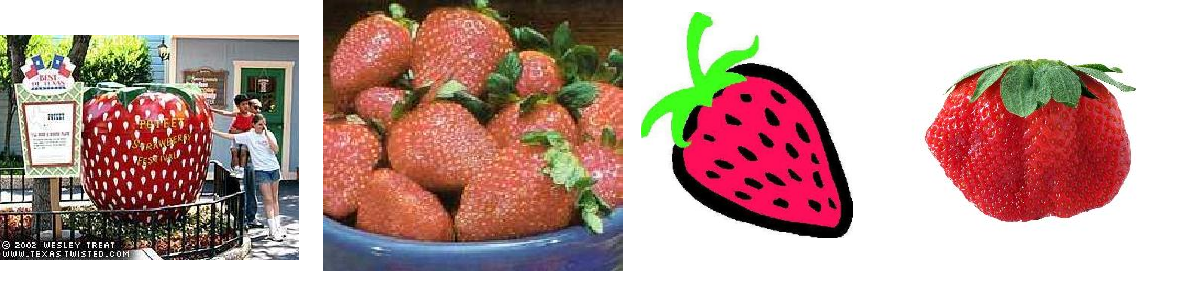
\includegraphics[scale=0.5]{images/strawberry.png}
	\caption{Verschiedene Bilder aus der Kategorie \enquote{Erdbeere} der Caltech101 Bilddaten.}
	\label{img:strawberries}
\end{figure}

\subsection{Testgenerierung}

Die Generierung von Testdaten bietet sich aus mehreren Gründen an. Zum einen sind enorm viele Trainingsdaten notwendig, um ein leistungsfähiges Modell zu generieren, zum anderen sollen im Test ca. 2000 Bildpaare verwendet werden. Ein manueller Testaufbau wäre fehleranfällig und nicht sehr flexibel. Da ein praktisch taugliches Modell erst durch die Variation einiger Parameter gefunden werden kann, ist es wünschenswert, Testdaten mit verschiedenen Eigenschaften generieren zu können:

\begin{itemize}
	\item Die Anzahl der Kategorien sollte bestimmbar sein. Dies entspricht einer Kategorie der Caltech101-Daten. Somit sind hier theoretisch bis zu 101 Kategorien im Test denkbar.
	\item Das Verhältnis bzw. die Anzahl an Trainings- und Testbildern muss definierbar sein.
\end{itemize}

Letztendlich sollen die Histogramme der \textit{Visual Words} zweier Bilder miteinander verglichen und so die Ähnlichkeit gemessen werden. Ein Programm automatisiert daher die Generierung solcher Paare: Es werden zufällige Bildpaare aus ausgewählten Kategorien (\textit{airplanes}, \textit{anchor}, ...) selektiert. Diese Paare, sowie die Information, ob die Bilder in der selben oder einer verschiedenen Kategorie liegen, stellen einen Testkandidaten dar. Zwei Bilder liegen dabei in der selben Klasse, wenn sie im selben Ordner im Dateisystem, also hier im Caltech101-Ordner, enthalten sind. Das Ergebnis wird dann als Datei \textit{test \textunderscore time.txt} gespeichert. Die Pfade der Bilder werden hierbei relativ zum Caltech101-Ordner gespeichert, die Information über die Kategorie wird als \enquote{+} bzw. \enquote{-} kodiert. Eine Datei für die Kategorien \textit{airplanes} und \textit{anchor} könnte dann so beginnen:\newline

\begin{lstlisting}
airplanes/image_0023.jpg airplanes/image_0009.jpg +
airplanes/image_0002.jpg anchor/image_0015.jpg -
anchor/image_0013.jpg airplanes/image_0002.jpg -
anchor/image_0001.jpg anchor/image_0005.jpg +
airplanes/image_0006.jpg anchor/image_0006.jpg -
...
\end{lstlisting}

Neben den zu verwendenden Kategorien muss bei Erzeugung die Anzahl der Testkandidaten, das Verhältnis von positiven zu negativen Kategorien sowie die Anzahl der Trainings- und Testbilder angegeben werden. \newline
Die Bilder, welche durch das Programm für das Training ausgewählt wurden, werden separat als \textit{train\textunderscore time.txt} gespeichert. Pro Zeile ist hier der relative Pfad des Bildes innerhalb des Caltech101-Ordners enthalten.

\section{Experimentaufbau}

Das Experiment soll sowohl die Feature-Kompression durch einen Autoencoder testen als auch die Kategorisierung bzw. den Vergleich der Bilder durch den Bag of Visual Words. Aus diesem Grund ist das Experiment zweigeteilt: 

\begin{enumerate}[(a)]%
	\item In dieser Variante findet ein reiner Test des Bag of Visual Words statt. Hierfür werden durch SIFT die Feature-Deskriptoren von Trainingsbildern extrahiert und direkt als Eingabe an den Bag of Visual Words gegeben. Anschließend folgt die Verarbeitung der Testbilder.
	\item Hier wird nach Extraktion der \textit{keypoints} durch den SIFT-Detektor der Feature-Deskriptor durch den Autoencoder erzeugt. Die so erhaltenen Features werden dann wie in (a) durch den Bag of Visual Words gruppiert und anschließend die \textit{Visual Words} der Testbilder erzeugt.
\end{enumerate}

Wichtig ist, dass pro Durchführung des Experiments in beiden Varianten die gleichen Trainings- und Testbilder verwendet werden, damit die Ergebnisse beider Deskriptoren miteinander vergleichbar sind. \newline
Nach Erzeugung des Modells mit den Trainingsbildern, werden nun die Features der Testkandidaten extrahiert und pro Bild dies \textit{Visual Words} berechnet. Die Ähnlichkeit \textit{sim (similarity)} der resultierenden Histogramme $h_1$ und $h_2$ wird dann als 1 $-$ \textit{MSE (mean squared error)} gemessen:

$$sim(h_1, h_2) = 1 - MSE(h_1, h_2)$$
$$MSE(h_1, h_2) = \frac{1}{n}\sum_{i=0}^{n}(h_{1_i} - h_{2_i})^{2}$$

\todo{Ergebnisse für alle Kandidaten nach sim sortieren. \enquote{Hohe Werte} (nah 1) sollten die gleiche Kategorie haben, geringe eine verschiedene} Hier gibt es zwei Fälle zu unterscheiden:

\begin{itemize}
	\item \textbf{True Positives} Bei \textit{True Positives} handelt es sich um zwei Bildern die entweder in der gleichen oder einer verschiedenen Klasse liegen und die Vorhersage des Modells diesbezüglich korrekt ist.
	\item \textbf{False Positives} In diesem Fall ist die Klassifizierung durch das Modell nicht korrekt: Bei gleicher Klasse wurde eine geringe Ähnlichkeit erkannt, bei verschiedenen eine Hohe.
\end{itemize}

Damit ein Modell zuverlässige Ergebnisse liefert, muss es größtenteils \textit{True Positives} erkennen, bzw. der Anteil der \textit{True Positives} sollte im Verhältnis zu den \textit{False Positives} bei weitem überwiegen. Für eine visuelle Darstellung dieses Verhältnisses eignet sich die \textit{Receiver Operating Characteristic (ROC)}: Diese stellt die \textit{True Positives} auf der Ordinate und die \textit{False-Positives} auf der Abzisse dar.

\section{Experimentdurchführung}

\todo{Auswertung für verschiedene k und beide Deskriptoren notieren. Das Ganze für drei verschieden Testsets. ROC Grafiken hinzufügen.}

\begin{table}
    \hfill
    \begin{tabular}[t]{ | r | c | c |}
    \hline
	     & SIFT & AE \\ \hline    
    5    & 0.00 & 0.00 \\ \hline
    10   & 0.00 & 0.00 \\ \hline
    20   & 0.00 & 0.00 \\ \hline
    50   & 0.00 & 0.00 \\ \hline
    100  & 0.00 & 0.00 \\ \hline
	250  & 0.00 & 0.00 \\ \hline
	500  & 0.00 & 0.00 \\ \hline
	1000 & 0.00 & 0.00 \\ \hline  
    \end{tabular}
    \hfill
    \begin{tabular}[t]{ | r | c | c |}
    \hline
	     & SIFT & AE \\ \hline    
    5    & 0.00 & 0.00 \\ \hline
    10   & 0.00 & 0.00 \\ \hline
    20   & 0.00 & 0.00 \\ \hline
    50   & 0.00 & 0.00 \\ \hline
    100  & 0.00 & 0.00 \\ \hline
	250  & 0.00 & 0.00 \\ \hline
	500  & 0.00 & 0.00 \\ \hline
	1000 & 0.00 & 0.00 \\ \hline    
    \end{tabular}
    \hfill
    \begin{tabular}[t]{ | r | c | c |}
    \hline
	     & SIFT & AE \\ \hline    
    5    & 0.00 & 0.00 \\ \hline
    10   & 0.00 & 0.00 \\ \hline
    20   & 0.00 & 0.00 \\ \hline
    50   & 0.00 & 0.00 \\ \hline
    100  & 0.00 & 0.00 \\ \hline
	250  & 0.00 & 0.00 \\ \hline
	500  & 0.00 & 0.00 \\ \hline
	1000 & 0.00 & 0.00 \\ \hline    
    \end{tabular}
    \hfill
	\caption{Laufzeiten der \textit{global memory} Implementierung des Bag of Visual Words. Von links nach rechts ist Test 1 bis 3 aufgelistet.}
\end{table}

\begin{table}
    \hfill
    \begin{tabular}[t]{ | r | c | c |}
    \hline
	     & SIFT & AE \\ \hline    
    5    & 0.00 & 0.00 \\ \hline
    10   & 0.00 & 0.00 \\ \hline
    20   & 0.00 & 0.00 \\ \hline
    50   & 0.00 & 0.00 \\ \hline
    90   & 0.00 & 0.00 \\ \hline
	200  & -    & 0.00 \\ \hline
	300  & -    & 0.00 \\ \hline    
    \end{tabular}
    \hfill
    \begin{tabular}[t]{ | r | c | c |}
    \hline
	     & SIFT & AE \\ \hline    
    5    & 0.00 & 0.00 \\ \hline
    10   & 0.00 & 0.00 \\ \hline
    20   & 0.00 & 0.00 \\ \hline
    50   & 0.00 & 0.00 \\ \hline
    90   & 0.00 & 0.00 \\ \hline
	200  & -    & 0.00 \\ \hline
	300  & -    & 0.00 \\ \hline
	\end{tabular}
    \hfill
    \begin{tabular}[t]{ | r | c | c |}
    \hline
	     & SIFT & AE \\ \hline    
    5    & 0.00 & 0.00 \\ \hline
    10   & 0.00 & 0.00 \\ \hline
    20   & 0.00 & 0.00 \\ \hline
    50   & 0.00 & 0.00 \\ \hline
    90   & 0.00 & 0.00 \\ \hline
	200  & -    & 0.00 \\ \hline
	300  & -    & 0.00 \\ \hline
	\end{tabular}
    \hfill
	\caption{Laufzeiten der \textit{shared memory} Implementierung des Bag of Visual Words. Von links nach rechts ist Test 1 bis 3 aufgelistet.}
\end{table}

\bibliographystyle{ieeetr}
\bibliography{sources}

\end{document}


